\subsubsection{Architettura ad alto livello-Monolith}
\label{Monolith}
\begin{figure}[H]
	\centering
	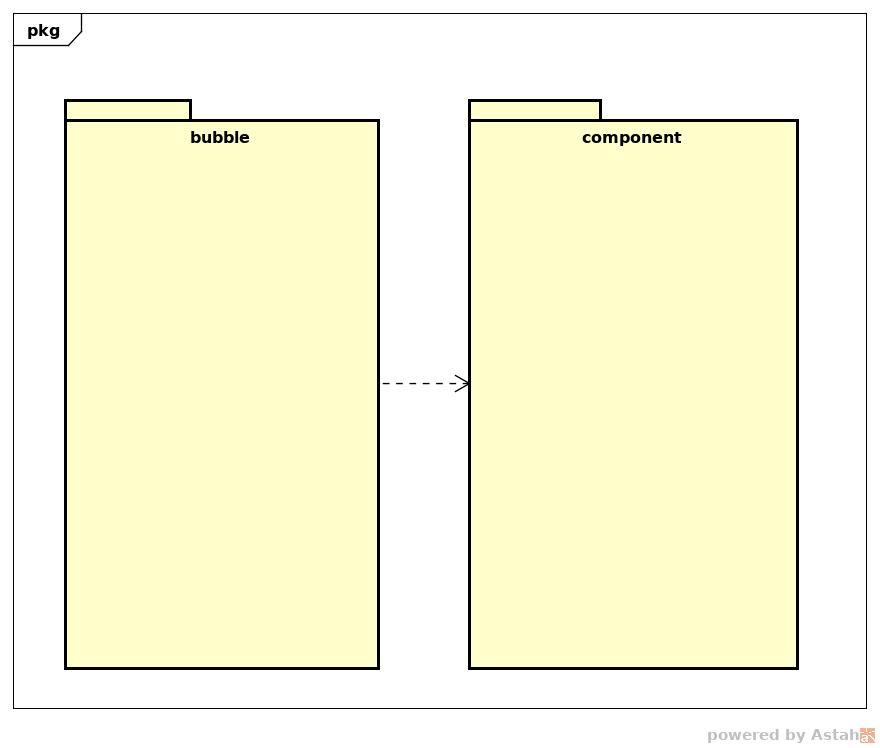
\includegraphics[scale=0.5]{Sezioni/Packages/SDK/Monolith.png}
	\caption{Architettura ad alto livello-Monolith}
\end{figure}
\begin{itemize}
	\item{\textbf{Descrizione}}: architettura ad alto livello dell’\termine{SDK} \termine{Monolith} del gruppo \gruppo. La struttura dei package scelta è quella classica dei progetti Meteor, però l'\termine{SDK} non possiede realmente una parte logica, per cui non è presente il package server poiché non necessario. Essendo, un'\termine{SDK} e rilasciato sotto licenza libera, è possibile che in un futuro vengano aggiunte nuove classi o ulteriori packages. A tal proposito il gruppo si è impegnato a suddividere le cartelle in modo da facilitare la disposizione e la ricerca delle componenti al suo interno.
	\item{\textbf{Package e classi contenuti}}:
	\begin{itemize}
	\item \textbf{client}: package contenente tutte le componenti necessarie al lato client.
	\end{itemize}

\end{itemize}

\subsection{Package monolith::client}

\label{Package monolith::client}
\begin{figure}[H]
	\centering
	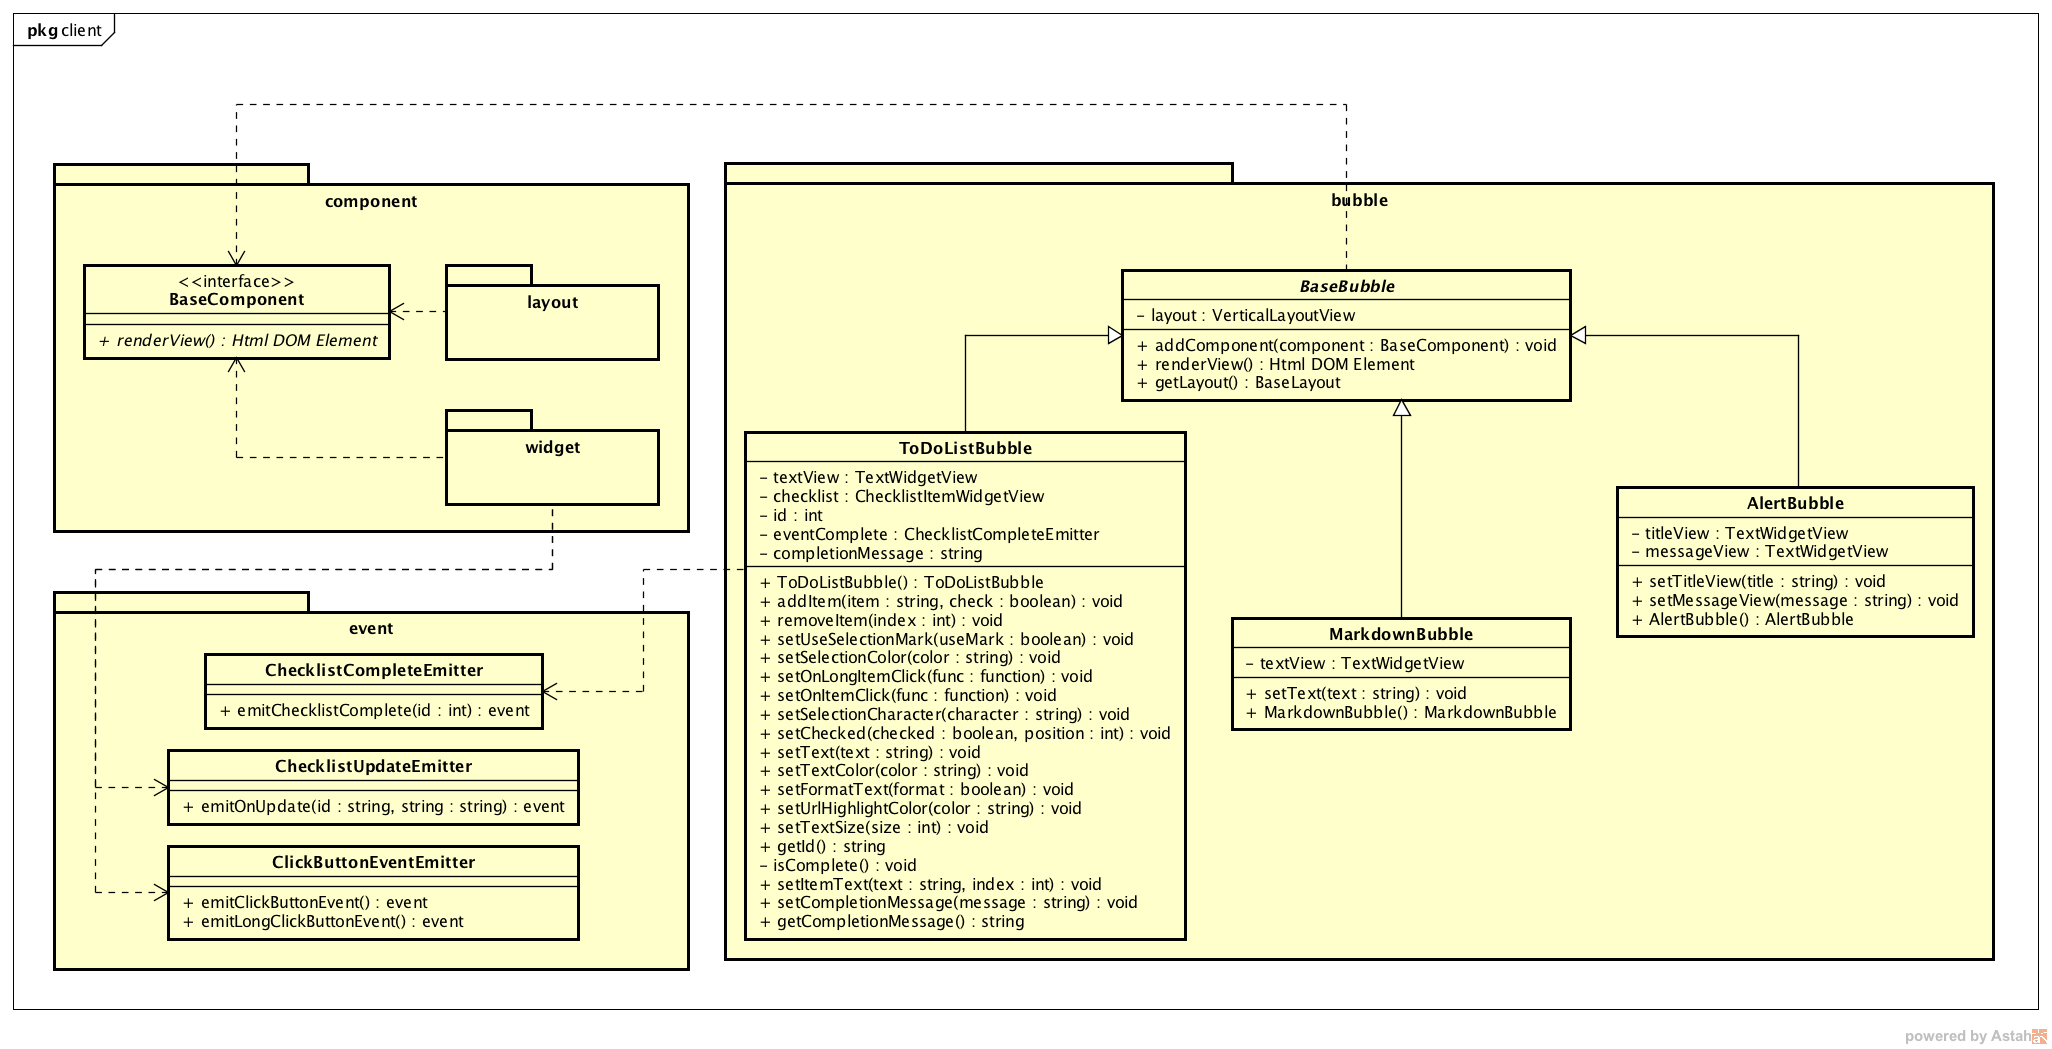
\includegraphics[width=16cm, height=8cm]{Sezioni/Packages/SDK/client.png}
	\caption{Package monolith::client}
\end{figure}

\begin{itemize}
\item \textbf{Descrizione}: package contenente le componenti adibite alle funzionalità lato client. 
\item \textbf{Classi e packages contenuti}:
\begin{itemize}
	\item \textbf{bubble}: package contenente tutti le componenti che rappresentano le bolle ed esso ha una dipendenza con il il package component. Le bolle, infatti, non sono altro che dei semplici contenitori che potranno contenere dei \textit{BaseComponent} (layout o widget) e disporli in qualsiasi logica si desideri. Infine, per considerare una componente una bolla, questa dovrà estendere la classe base \textit{BaseBubble}, classe base della gerarchia.
	\item \textbf{component}: package contenente tutti i package dei componenti che compongono le bolle, ad esempio tutti i tipi di widget e layout. Questi possono essere aggiunti alle bolle e, aggiungere un layout significa introdurre in una bolla una logica di disposizione degli elementi. Si noti, infine, che una \termine{BaseBubble} (punto di partenza per qualsiasi bolla) per scelta implementativa possiede di default un layout verticale.
	\item \textbf{BaseComponent}: interfaccia che rappresenta un generico componente. Qualsiasi classe adibita a questa funzionalità dovrà implementare (o estendere) questa interfaccia.
\end{itemize}
\end{itemize}

\subsubsection{Package monolith::client::component}
\label{Package monolith::client::component}
\begin{figure}[H]
	\centering
	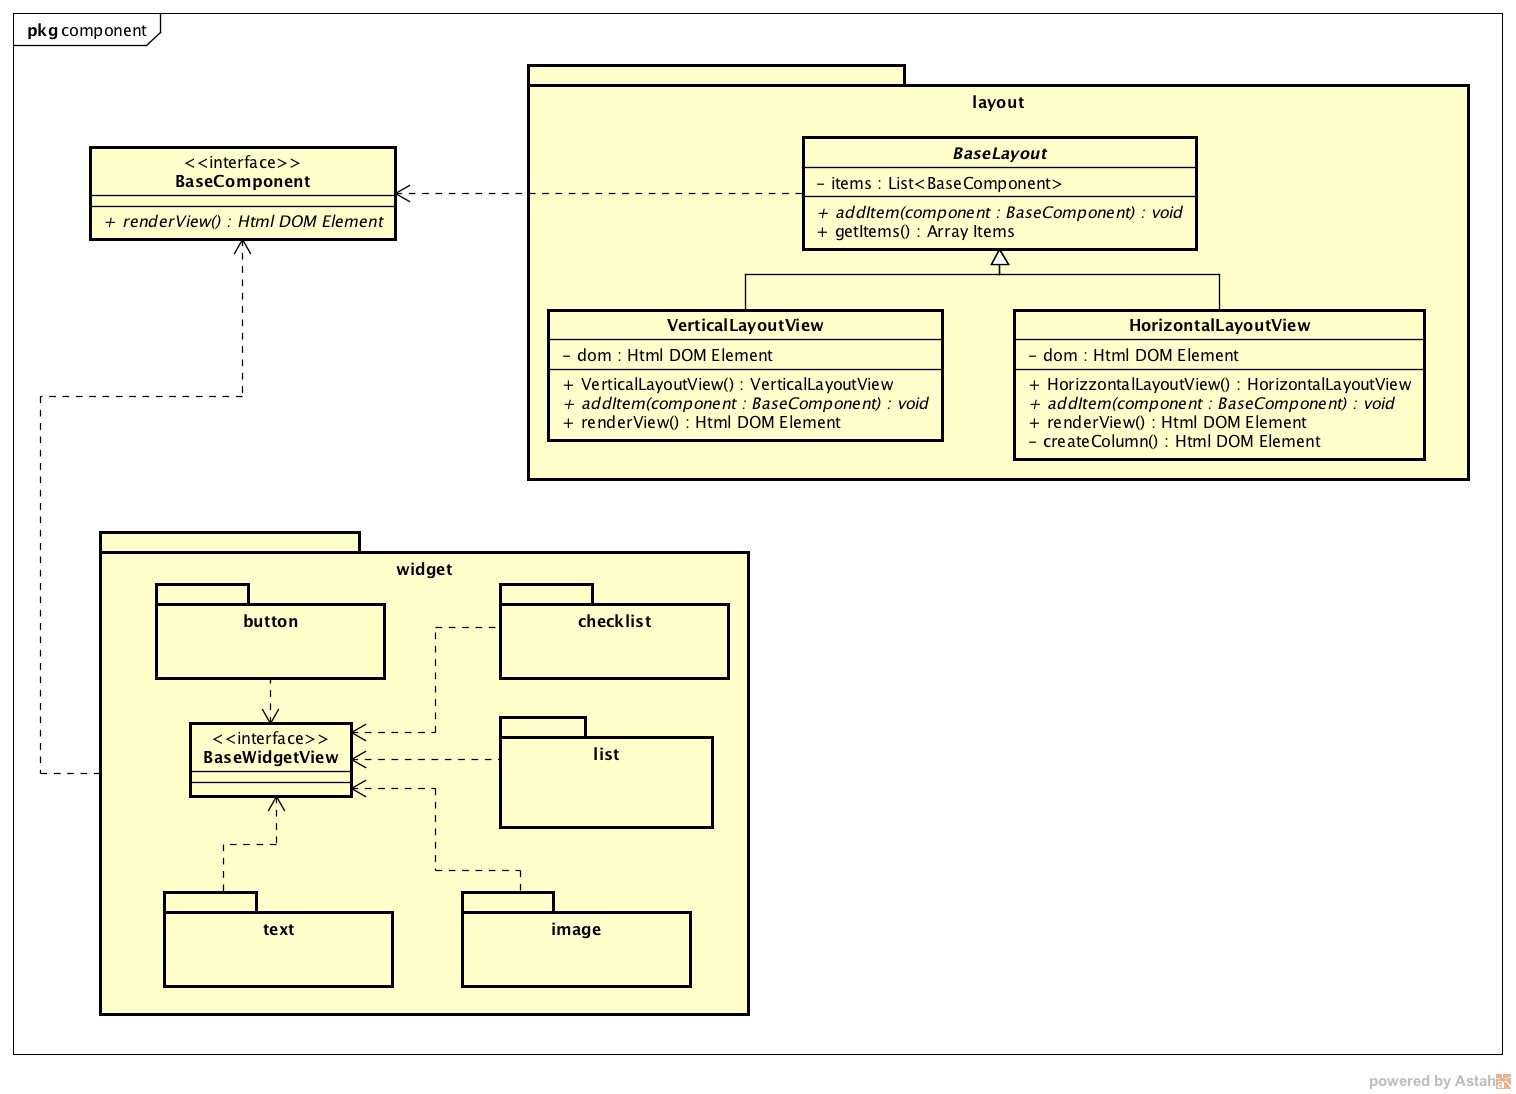
\includegraphics[width=\textwidth]{Sezioni/Packages/SDK/component.png}
	\caption{Package monolith::client::component}
\end{figure}

\begin{itemize}
\item \textbf{Descrizione}: package contenente altri due packages. Il primo contiene i widget, il secondo i layout. Essi sono entrambi dei component poiché possono essere aggiunti a qualsiasi bolla per garantire più libertà di modifica possibile. Infatti, una bolla può essere formata da più layout contenenti ognuno varie componenti.
Si noti che i widget sono considerati dei \textit{BaseComponent} per cui ognuno di essi ha una dipendenza con l'interfaccia. Per comodità tale dipendenza è espressa a livello del package esterno.
\item \textbf{Classi e packages contenuti}:
\begin{itemize}
\item \textbf{layout}: package che contiene le componenti che forniscono le funzionalità dei layout. Essi vengono usati per disporre i widget nelle \termine{bolle}.
\item \textbf{widget}: package che contiene i widget, ovvero le componenti che formano effettivamente le \termine{bolle}.
\item \textbf{BaseComponent}: interfaccia che rappresenta la base degli oggetti che possono essere aggiunti ad una \termine{bolla}.
\end{itemize}
\end{itemize}

\subsubsection{Package monolith::client::component::widget::button}
\label{Package monolith::client::component::widget::button}
\begin{figure}[H]
	\centering
	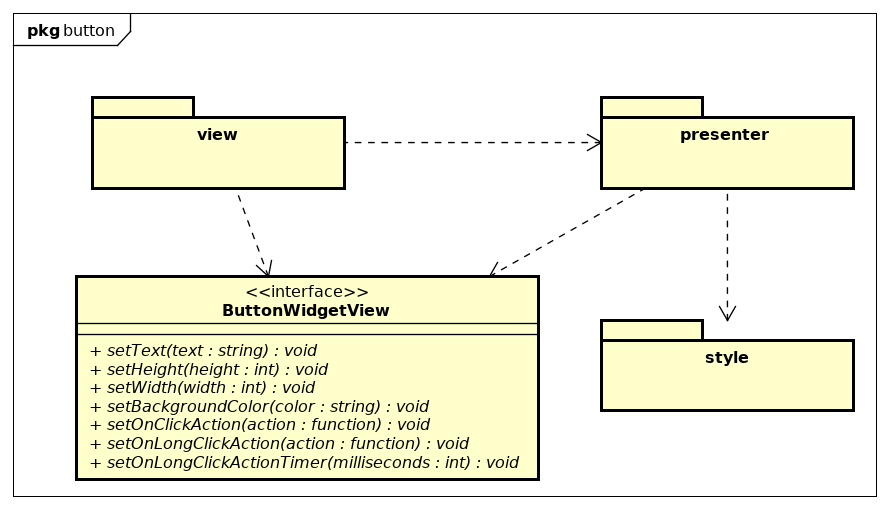
\includegraphics[scale=0.5]{Sezioni/Packages/SDK/button.png}
	\caption{Package monolith::client::component::widget::button}
\end{figure}
\begin{itemize}
\item \textbf{Descrizione}: package contenente altri package che rappresentano la componente widget bottone. 
\item \textbf{Classi e packages contenuti}:
\begin{itemize}
\item \textbf{view}: package che contiene le implementazioni dell'interfaccia \textit{ButtonWidgetView}.
\item \textbf{presenter}: package che contiene il/ i presenter del widget bottone.
\item \textbf{style}: package contenente la classe (o le classi, nel caso se ne definiscano di più) che incapsulano le informazioni o gli attributi del widget bottone.
\item \textbf{ButtonWidgetView}: interfaccia che rappresenta la view da implementare del widget bottone.
\end{itemize}
\end{itemize}

\subsubsection{Package monolith::client::component::widget::checklist}
\label{Package monolith::client::component::widget::checklist}
\begin{figure}[H]
	\centering
	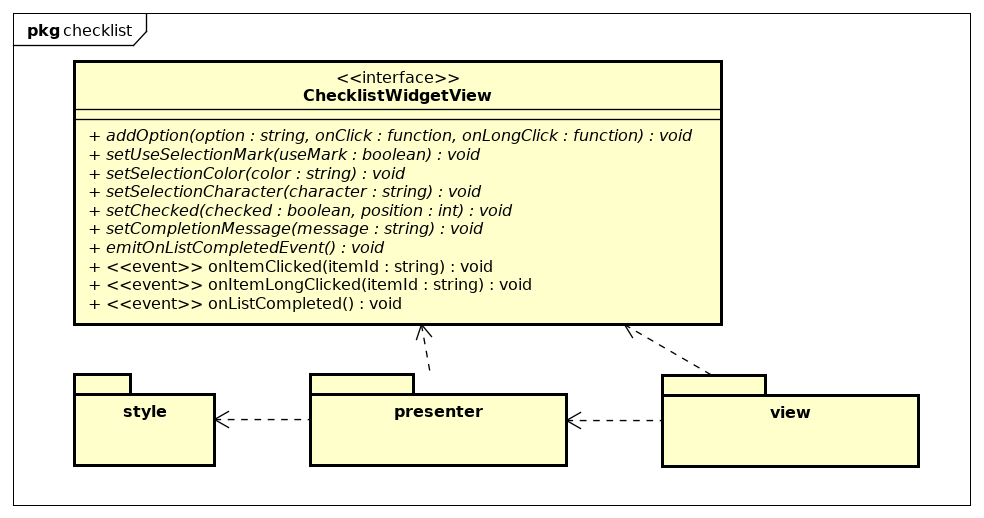
\includegraphics[scale=0.5]{Sezioni/Packages/SDK/checklist.png}
	\caption{Package monolith::client::component::widget::checklist}
\end{figure}
\begin{itemize}
\item \textbf{Descrizione}: package contenente altri package che rappresentano la componente widget checklist.
\item \textbf{Classi e packages contenuti}:
\begin{itemize}
\item \textbf{view}: package che contiene le implementazioni dell'interfaccia \textit{ChecklistWidgetView}.
\item \textbf{presenter}: package che contiene il/ i presenter del widget checklist.
\item \textbf{style}: package contenente la classe (o le classi, nel caso se ne definiscano di più) che incapsulano le informazioni o gli attributi del widget checklist.
\item \textbf{ChecklistWidgetView}: interfaccia che rappresenta la view da implementare del widget checklist.
\end{itemize}
\end{itemize}

\subsubsection{Package monolith::client::component::widget::list}
\label{Package monolith::client::component::widget::list}
\begin{figure}[H]
	\centering
	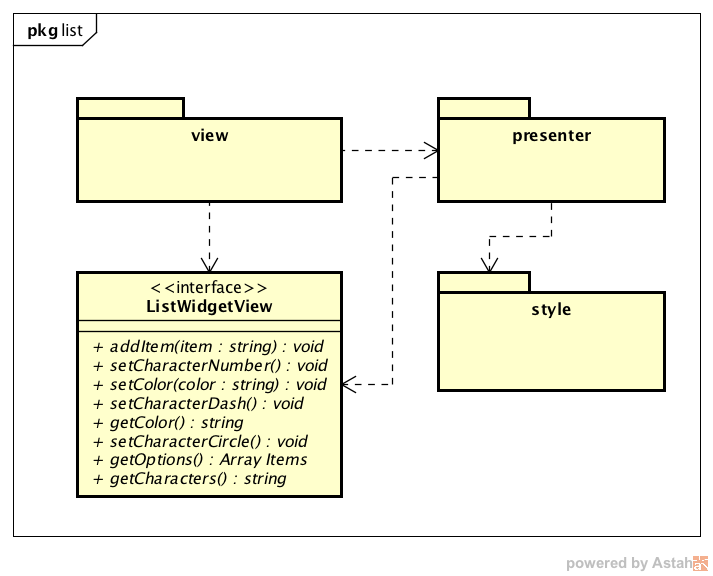
\includegraphics[scale=0.5]{Sezioni/Packages/SDK/list.png}
	\caption{Package monolith::client::component::widget::list}
\end{figure}
\begin{itemize}
\item \textbf{Descrizione}: package contenente altri package che rappresentano la componente lista generica.
\item \textbf{Classi e packages contenuti}:
\begin{itemize}
\item \textbf{view}: package che contiene le implementazioni dell'interfaccia \textit{ListWidgetView}.
\item \textbf{presenter}: package che contiene il/ i presenter della lista generica.
\item \textbf{style}: package contenente la classe (o le classi, nel caso se ne definiscano di più) che incapsulano le informazioni o gli attributi della lista generica.
\item \textbf{ListWidgetView}: interfaccia che rappresenta la view da implementare della List.
\end{itemize}
\end{itemize}

\subsubsection{Package monolith::client::component::widget::image}
\label{Package monolith::client::component::widget:image}
\begin{figure}[H]
	\centering
	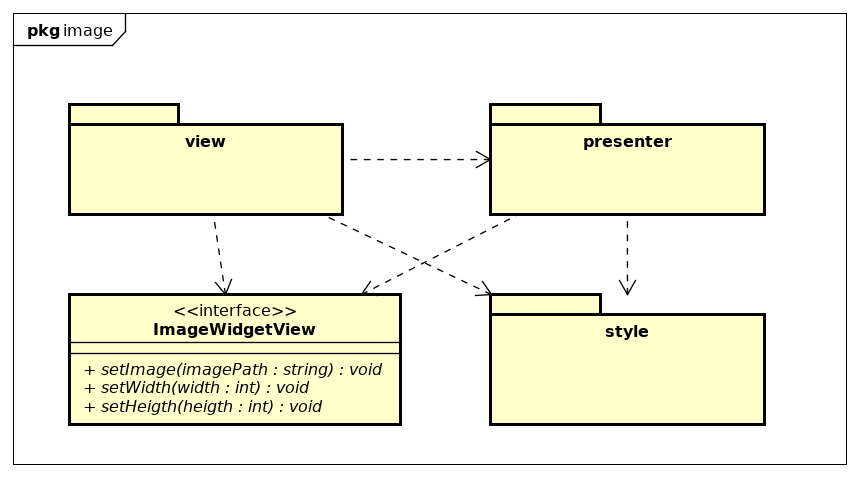
\includegraphics[scale=0.5]{Sezioni/Packages/SDK/image.png}
	\caption{Package monolith::client::component::widget::image}
\end{figure}
\begin{itemize}
\item \textbf{Descrizione}: package contenente altri package che rappresentano la componente widget immagine.
\item \textbf{Classi e packages contenuti}:
\begin{itemize}
\item \textbf{view}: package che contiene le implementazioni dell'interfaccia \textit{ImageWidgetView}.
\item \textbf{presenter}: package che contiene il/ i presenter del widget immagine.
\item \textbf{style}: package contenente la classe (o le classi, nel caso se ne definiscano di più) che incapsulano le informazioni o gli attributi del widget immagine.
\item \textbf{ImageWidgetView}: interfaccia che rappresenta la view da implementare del widget immagine.
\end{itemize}
\end{itemize}

\subsubsection{Package monolith::client::component::widget::text}
\label{Package monolith::client::component::widget::text}
\begin{figure}[H]
	\centering
	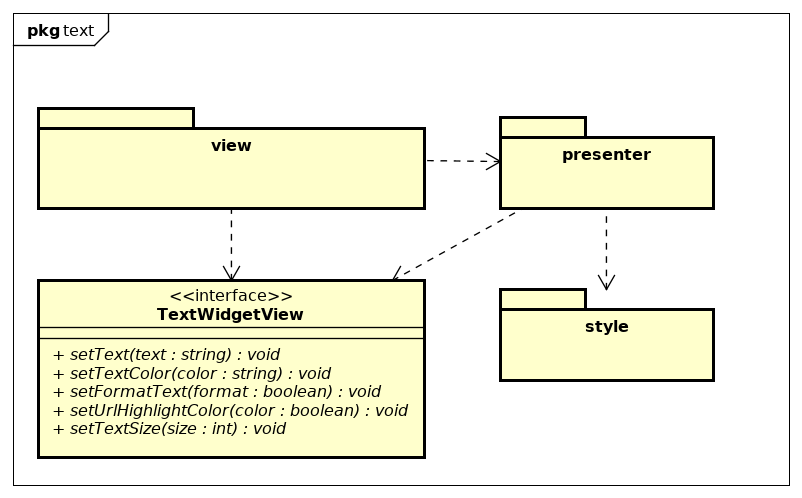
\includegraphics[scale=0.5]{Sezioni/Packages/SDK/text.png}
	\caption{Package monolith::client::component::widget::text}
\end{figure}
\begin{itemize}
\item \textbf{Descrizione}: package contenente altri package che rappresentano la componente widget testo.
\item \textbf{Classi e packages contenuti}:
\begin{itemize}
\item \textbf{view}: package che contiene le implementazioni dell'interfaccia \textit{TextWidgetView}.
\item \textbf{presenter}: package che contiene il/ i presenter del widget testo.
\item \textbf{style}: package contenente la classe (o le classi, nel caso se ne definiscano di più) che incapsulano le informazioni o gli attributi del widget testo.
\item \textbf{TextWidgetView}: interfaccia che rappresenta la view da implementare del widget testo.
\end{itemize}
\end{itemize}



































\begin{comment}
\subsubsection{Suddivisione in package  di Monolith::bubble}
\label{Monolith::bubble}
\begin{figure}[H]
	\centering
	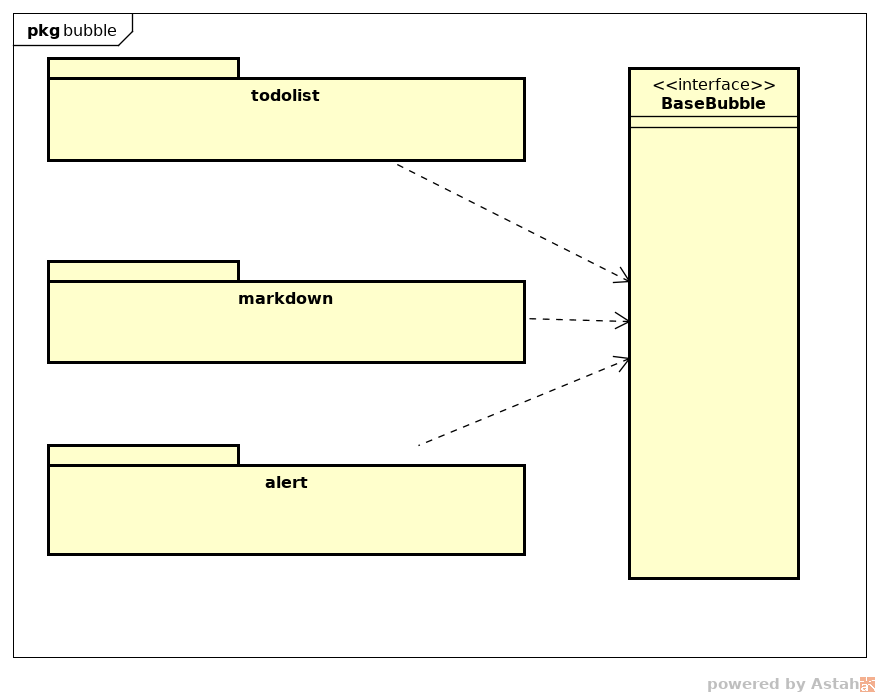
\includegraphics[scale=0.5]{Sezioni/Packages/SDK/bubble.png}
	\caption{Monolith::bubble}
\end{figure}
\begin{itemize}
	\item{\textbf{Descrizione}}: packege contenente tutti i tipi di bolle del \termine{SDK}.
	\item{\textbf{Package e classi contenuti}}:
	\begin{itemize}
	\item{monolith::bubble::todolist}: package contenente la classe per creare una bolla di tipo ToDoList.
	\item{monolith::component::markdown}: package contenente la classe per creare una bolla di tipo \termine{markdown}.
	\item{monolith::component::alert}: package contenente la classe per creare una bolla di tipo alert.

	\end{itemize}

\end{itemize}

\subsubsection{Suddivisione in package  di Monolith::bubble::todolist}
\label{Monolith::bubble::todolist}
\begin{figure}[H]
	\centering
	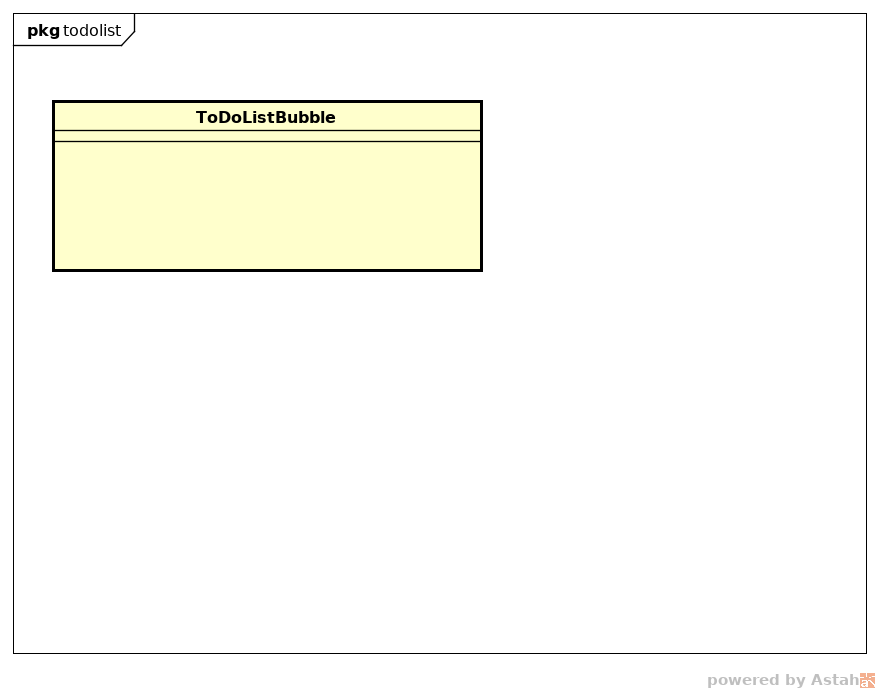
\includegraphics[scale=0.5]{Sezioni/Packages/SDK/bubble_todolist.png}
	\caption{Monolith::todolist}
\end{figure}
\begin{itemize}
	\item{\textbf{Descrizione}}: package contenente la classe per creare la bolla di tipo ToDoList
	\item{\textbf{Classi contenuti}}:
	\begin{itemize}
	\item{monolith::bubble::ToDoListBubble}: classe per creare la bolla di tipo ToDoList.
	\end{itemize}
\end{itemize}

\subsubsection{Suddivisione in package  di Monolith::bubble::markdown}
\label{Monolith::bubble::markdown}
\begin{figure}[H]
	\centering
	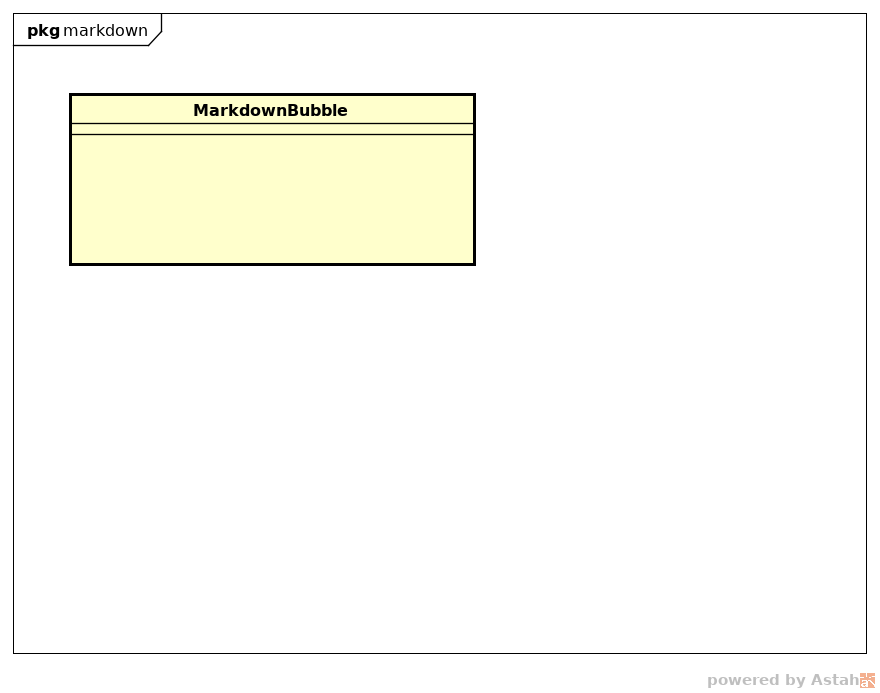
\includegraphics[scale=0.5]{Sezioni/Packages/SDK/bubble_markdown.png}
	\caption{Monolith::markdown}
\end{figure}
\begin{itemize}
	\item{\textbf{Descrizione}}: package contenente la classe per creare la bolla di tipo \termine{Markdown}
	\item{\textbf{Classi contenuti}}:
	\begin{itemize}
	\item{monolith::bubble::MarkDownBubble}: classe per creare la bolla di tipo \termine{MarkDown}.
	\end{itemize}
\end{itemize}

	\subsubsection{Suddivisione in package  di Monolith::bubble::alert}
\label{Monolith::bubble::alert}
\begin{figure}[H]
	\centering
	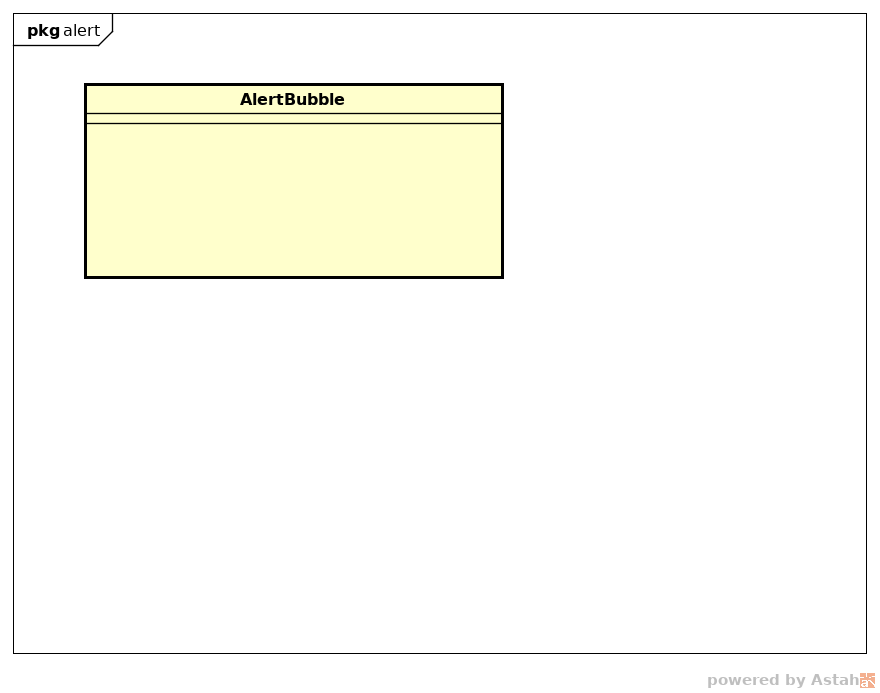
\includegraphics[scale=0.5]{Sezioni/Packages/SDK/bubble_alert.png}
	\caption{Monolith::bubble::alert}
\end{figure}
\begin{itemize}
	\item{\textbf{Descrizione}}: package contenente la classe per creare la bolla di tipo Alert
	\item{\textbf{Package e classi contenuti}}:
	\begin{itemize}
	\item{monolith::bubble::AlertBubble}: classe per creare la bolla di tipo Alert.
	\end{itemize}
\end{itemize}



\subsubsection{Suddivisione in package  di Monolith::component}
\label{Monolith::component}
\begin{figure}[H]
	\centering
	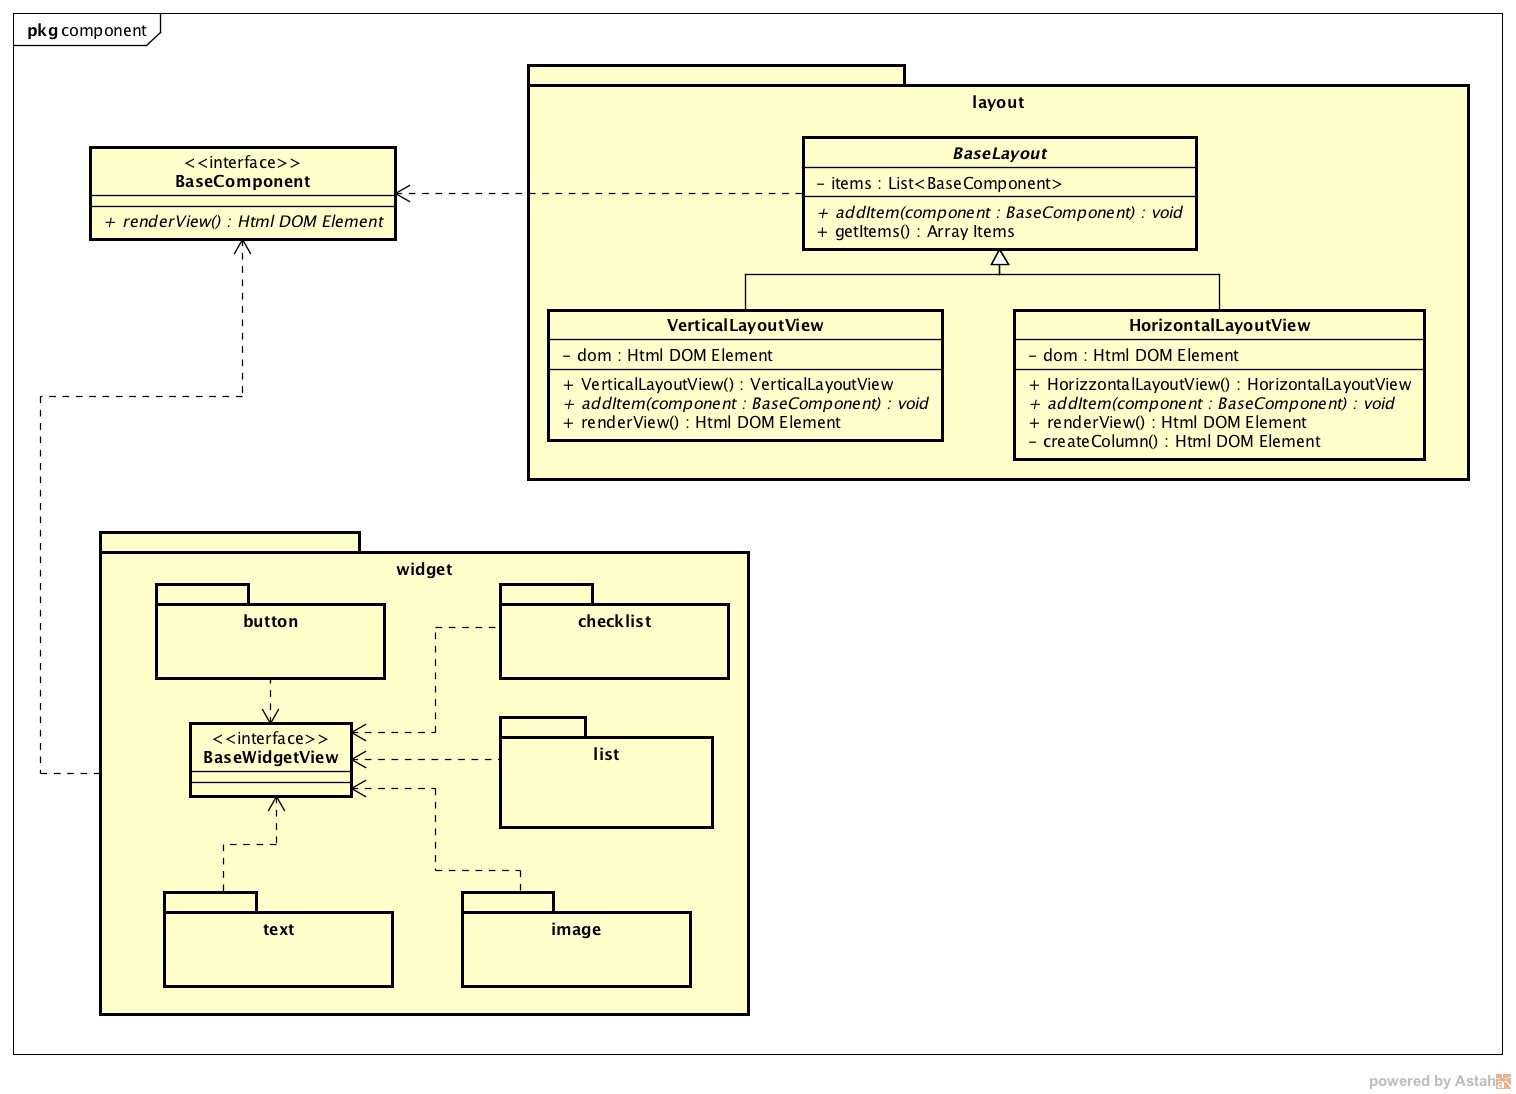
\includegraphics[scale=0.5]{Sezioni/Packages/SDK/component.png}
	\caption{Monolith::component}
\end{figure}
\begin{itemize}
	\item{\textbf{Descrizione}}: package contenente tutti i packages che permettono la creazione dei componenti di una bolla.
	\item{\textbf{Package e classi contenuti}}:
	\begin{itemize}
	\item{monolith::component::layout}: package contenente tutti i package e le classi per la creazione di un layout, esso ha la una dipendenza tra i \termine{widget}.
	\item{monolith::component::widget}: package contenente tutti i package per la creazione di un \termine{widget}.
	\item{monolith::component::BaseComponent}: interfaccia per un component base.
	\end{itemize}

\end{itemize}

\subsubsection{Suddivisione in package  di Monolith::component::layout}
\label{Monolith::component::layout}
\begin{figure}[H]
	\centering
	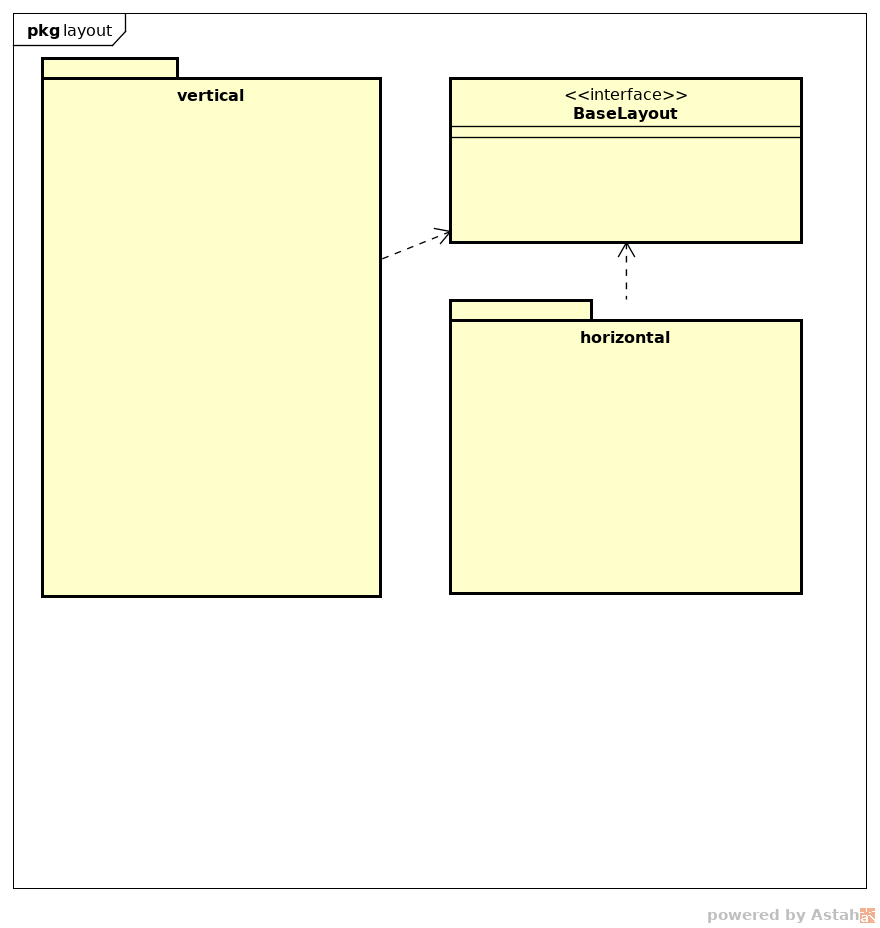
\includegraphics[scale=0.5]{Sezioni/Packages/SDK/component_layout.png}
	\caption{Monolith::component::layout}
\end{figure}
\begin{itemize}
	\item{\textbf{Descrizione}}: package contenente tutti i packages e le classi che permettono la creazione di un layout.
	\item{\textbf{Package e classi contenuti}}:
	\begin{itemize}
	\item{monolith::component::layout::vertical}: package contenente tutti i package e le classi per la creazione di un layout verticale.
	\item{monolith::component::layout::horizontal}: package contenente tutti i package e le classi per la creazione di un layout orizzontale.
	\item{monolith::component::layout:BaseLayout}: interfaccia per un layout base.
	\end{itemize}

\end{itemize}


\subsubsection{Suddivisione in package  di Monolith::component::layout::vertical}
\label{Monolith::component::layout::vertical}
\begin{figure}[H]
	\centering
	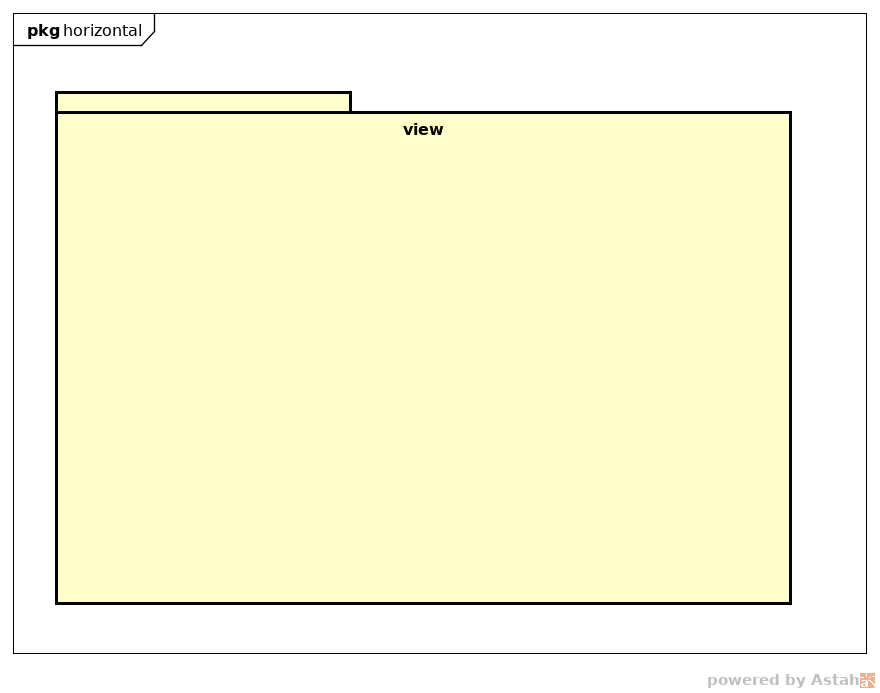
\includegraphics[scale=0.5]{Sezioni/Packages/SDK/component_layout_vertical.png}
	\caption{Monolith::component::layout::vertical}
\end{figure}
\begin{itemize}
	\item{\textbf{Descrizione}}: package contenente il package view per creare un layout verticale.
	\item{\textbf{Classi contenuti}}:
	\begin{itemize}
	\item{monolith::component::layout::vertical::view}: package contentente la view per la creazione di un layout verticale.
	\end{itemize}
\end{itemize}

\subsubsection{Suddivisione in package  di Monolith::component::layout::horizontal}
\label{Monolith::component::layout::horizontal}
\begin{figure}[H]
	\centering
	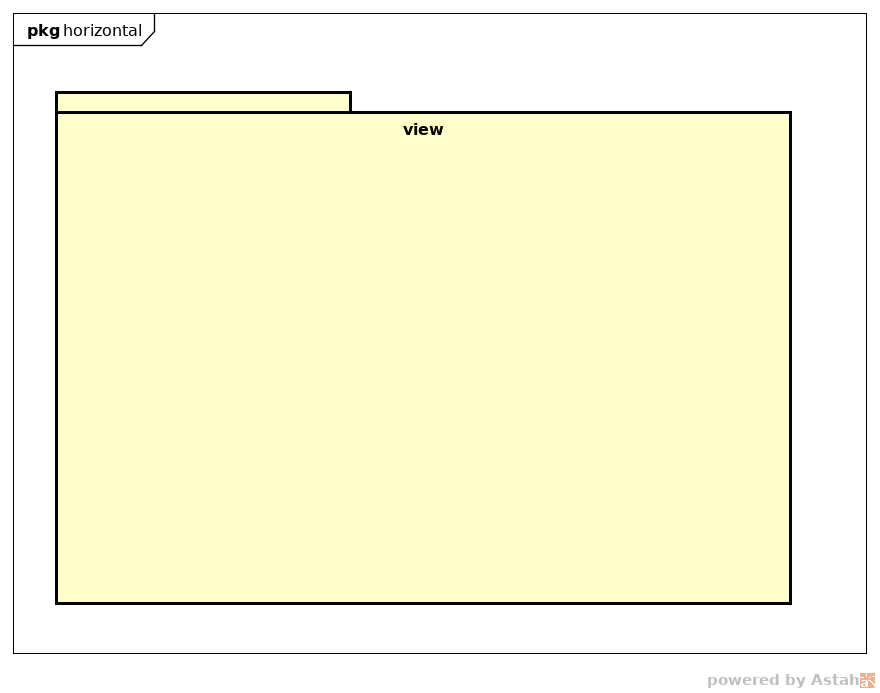
\includegraphics[scale=0.5]{Sezioni/Packages/SDK/component_layout_horizontal.png}
	\caption{Monolith::component::layout::horizontal}
\end{figure}
\begin{itemize}
	\item{\textbf{Descrizione}}: package contenente il package view per creare un layout orizzontale.
	\item{\textbf{Classi contenuti}}:
	\begin{itemize}
	\item{monolith::component::layout::horizontal::view}: package contentente la view per la creazione di un layout orizzontale.
	\end{itemize}
\end{itemize}

\subsubsection{Suddivisione in package  di Monolith::component::layout::horizontal:view}
\label{Monolith::component::layout::horizontal::view}
\begin{figure}[H]
	\centering
	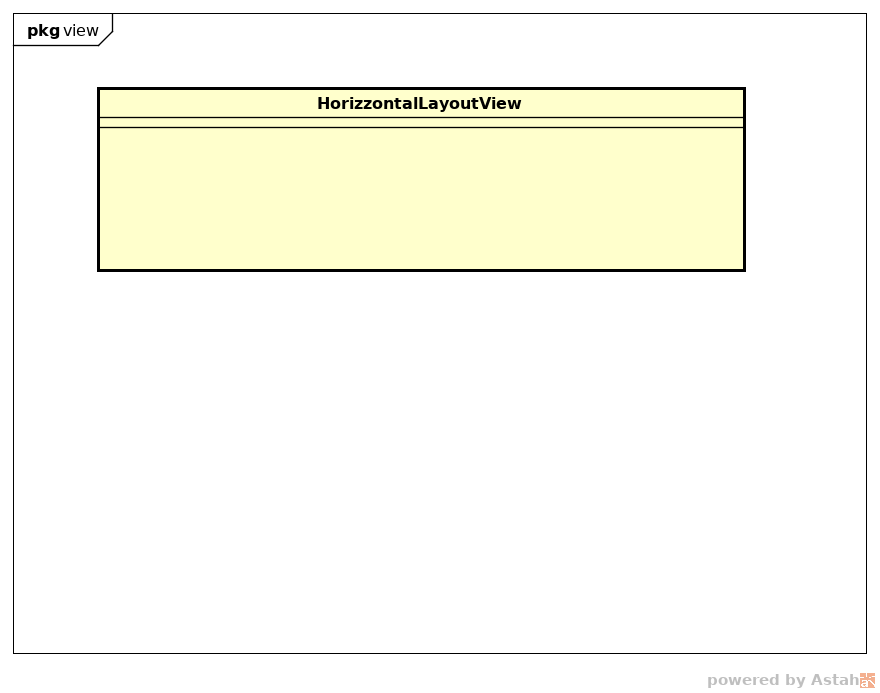
\includegraphics[scale=0.5]{Sezioni/Packages/SDK/component_layout_horizontal_view.png}
	\caption{Monolith::component::layout::horizontal::view}
\end{figure}
\begin{itemize}
	\item{\textbf{Descrizione}}: package contenente la classe view per creare un layout orizzontale.
	\item{\textbf{Classi contenuti}}:
	\begin{itemize}
	\item{monolith::component::layout::horizontal::view::HorizontalLayoutView}: classe view per la creazione di un layout orizzontale.
	\end{itemize}
\end{itemize}

\subsubsection{Suddivisione in package  di Monolith::component::layout::vertical:view}
\label{Monolith::component::layout::vertical::view}
\begin{figure}[H]
	\centering
	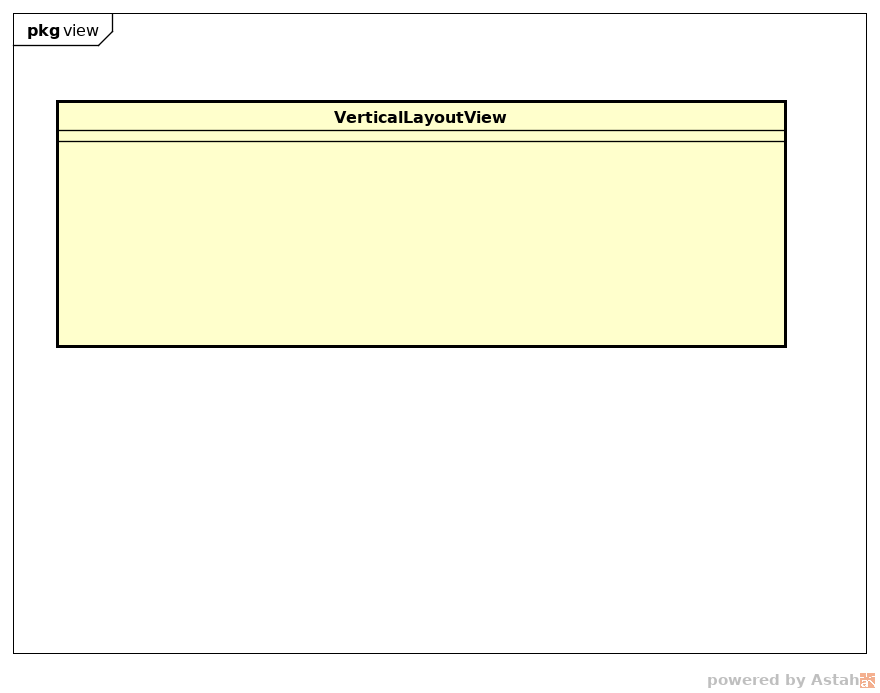
\includegraphics[scale=0.5]{Sezioni/Packages/SDK/component_layout_vertical_view.png}
	\caption{Monolith::component::layout::vertical::view}
\end{figure}
\begin{itemize}
	\item{\textbf{Descrizione}}: package contenente la classe view per creare un layout verticale.
	\item{\textbf{Classi contenuti}}:
	\begin{itemize}
	\item{monolith::component::layout::vertical::view::VerticalLayoutView}: classe view per la creazione di un layout verticale.
	\end{itemize}
\end{itemize}

\subsubsection{Suddivisione in package  di Monolith::component::widget}
\label{Monolith::component::widget}
\begin{figure}[H]
	\centering
	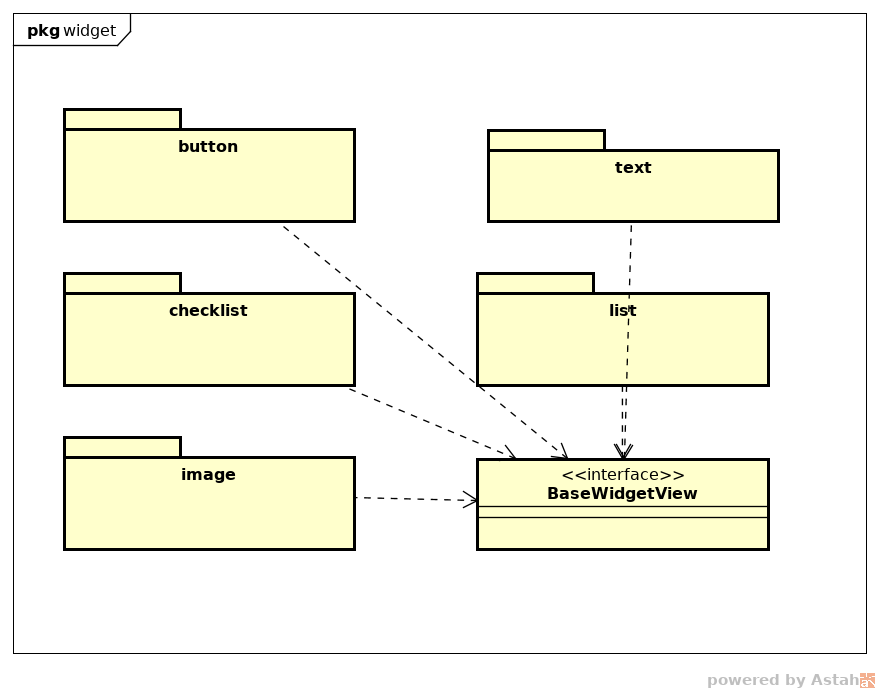
\includegraphics[scale=0.5]{Sezioni/Packages/SDK/component_widget.png}
	\caption{Monolith::component::widget}
\end{figure}
\begin{itemize}
	\item{\textbf{Descrizione}}: package contenente tutti i packages e le classi che permettono la creazione di un \termine{widget}.
	\item{\textbf{Package e classi contenuti}}:
	\begin{itemize}
	\item{monolith::component::widget::button}: package contenente tutti i package e le classi per la creazione di un widget botton.
	\item{monolith::component::widget::text}: package contenente tutti i package e le classi per la creazione di un widget text, ha una dipendenza con l'interfaccia BaseWidgetView.
	\item{monolith::component::widget::checklist}: package contenente tutti i package e le classi per la creazione di un widget checklist, ha una dipendenza con l'interfaccia BaseWidgetView.
	\item{monolith::component::widget::list}: package contenente tutti i package e le classi per la creazione di un widget list, ha una dipendenza con l'interfaccia BaseWidgetView.
	\item{monolith::component::widget::image}: package contenente tutti i package e le classi per la creazione di un widget image, ha una dipendenza con l'interfaccia BaseWidgetView.
	\item{monolith::component::widget::BaseWidget}: interfaccia per un widget base.
	\end{itemize}

\end{itemize}

\subsubsection{Suddivisione in package  di Monolith::component::widget::button}
\label{Monolith::component::widget::button}
\begin{figure}[H]
	\centering
	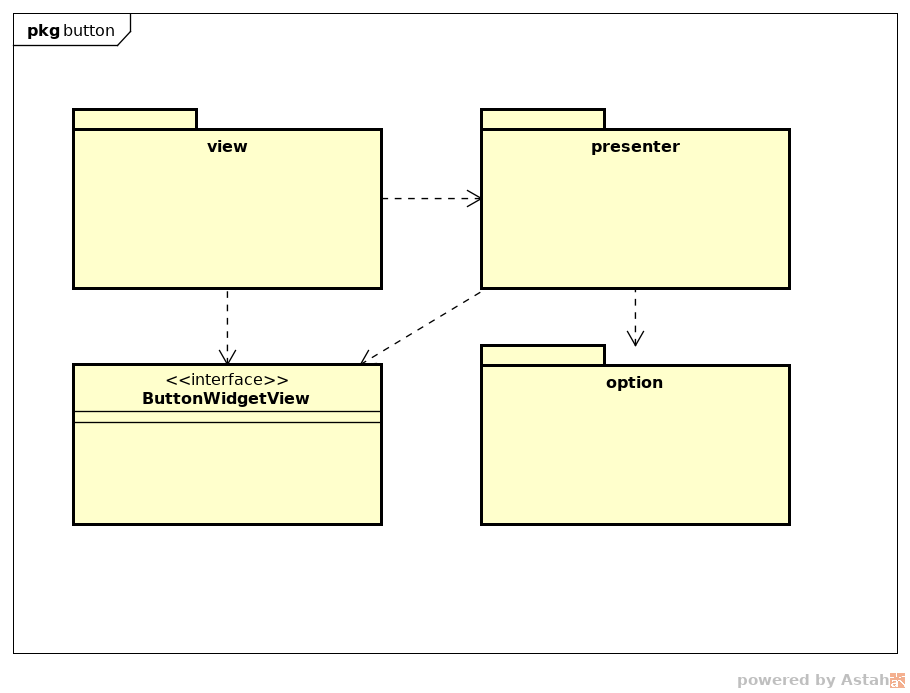
\includegraphics[scale=0.5]{Sezioni/Packages/SDK/component_widget_button.png}
	\caption{Monolith::component::widget::button}
\end{figure}
\begin{itemize}
	\item{\textbf{Descrizione}}: package contenente tutti i packages e le classi che permettono la creazione di un widget button.
	\item{\textbf{Package e classi contenuti}}:
	\begin{itemize}
	\item{monolith::component::widget::button::view}: package contenente tutte le classi per la view di un widget button.
	\item{monolith::component::widget::button::presenter}: package contenente tutte le classi per il presenter di un widget button.
	\item{monolith::component::widget::button::option}: package contenente tutte le classi per le option di un widget button.
	\item{monolith::component::widget::ButtonWidgetView}: interfaccia per un widget button.
	\end{itemize}

\end{itemize}


\subsubsection{Suddivisione in package  di Monolith::component::widget::button::view}
\label{monolith::component::widget::button::view}
\begin{figure}[H]
	\centering
	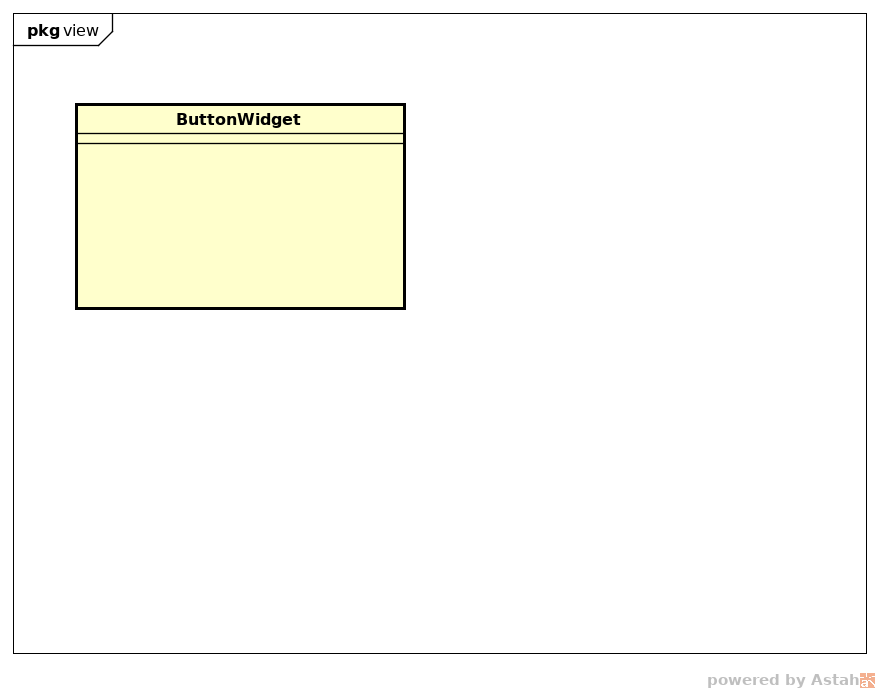
\includegraphics[scale=0.5]{Sezioni/Packages/SDK/component_widget_button_view.png}
	\caption{monolith::component::widget::button::view}
\end{figure}
\begin{itemize}
	\item{\textbf{Descrizione}}: package contenente la classe view per creare un widget button.
	\item{\textbf{Classi contenuti}}:
	\begin{itemize}
	\item{monolith::component::widget::button::view::ButtonWidget}: classe view per la creazione di un widget button.
	\end{itemize}
\end{itemize}


\subsubsection{Suddivisione in package  di Monolith::component::widget::button::presenter}
\label{monolith::component::widget::button::presenter}
\begin{figure}[H]
	\centering
	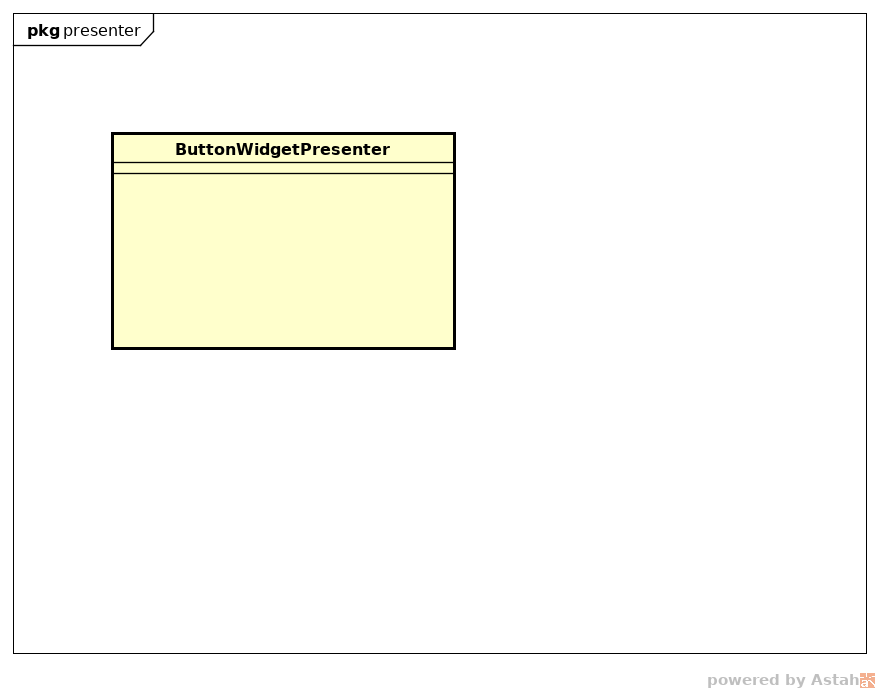
\includegraphics[scale=0.5]{Sezioni/Packages/SDK/component_widget_button_presenter.png}
	\caption{onolith::component::widget::button::presenter}
\end{figure}
\begin{itemize}
	\item{\textbf{Descrizione}}: package contenente la classe presenter per creare un widget button.
	\item{\textbf{Classi contenuti}}:
	\begin{itemize}
	\item{monolith::component::widget::button::presenter::ButtonWidgetPresenter}: classe presenter per la creazione di un widget button.
	\end{itemize}
\end{itemize}



\subsubsection{Suddivisione in package  di Monolith::component::widget::button::option}
\label{monolith::component::widget::button::option}
\begin{figure}[H]
	\centering
	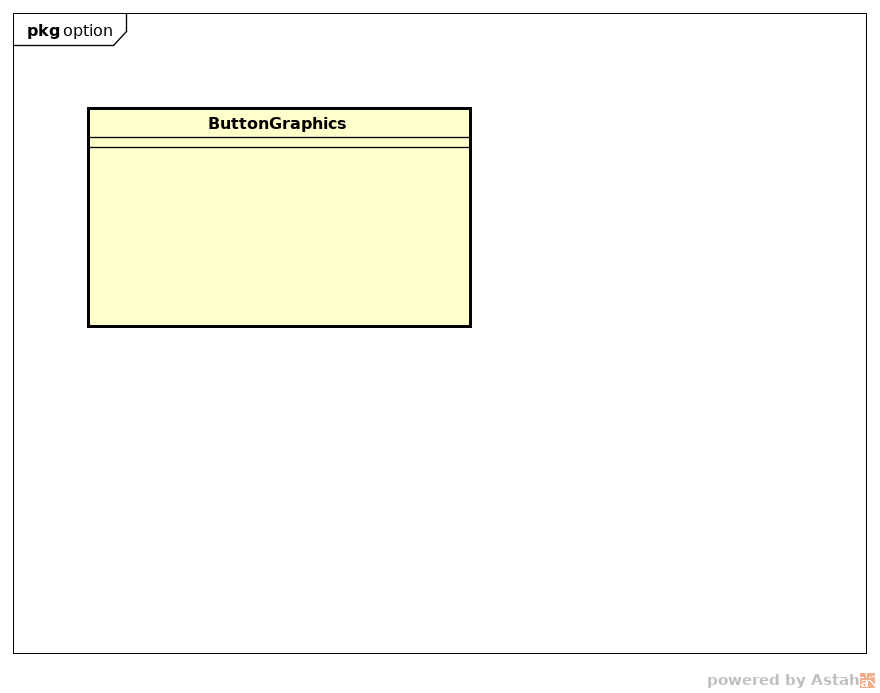
\includegraphics[scale=0.5]{Sezioni/Packages/SDK/component_widget_button_option.png}
	\caption{monolith::component::widget::button::option}
\end{figure}
\begin{itemize}
	\item{\textbf{Descrizione}}: package contenente la classe option per creare un widget button.
	\item{\textbf{Classi contenuti}}:
	\begin{itemize}
	\item{monolith::component::widget::button::option::ButtonGraphics}: classe per la modifica della grafica di un widget button.
	\end{itemize}
\end{itemize}

\subsubsection{Suddivisione in package  di Monolith::component::widget::checklist}
\label{Monolith::component::widget::checklist}
\begin{figure}[H]
	\centering
	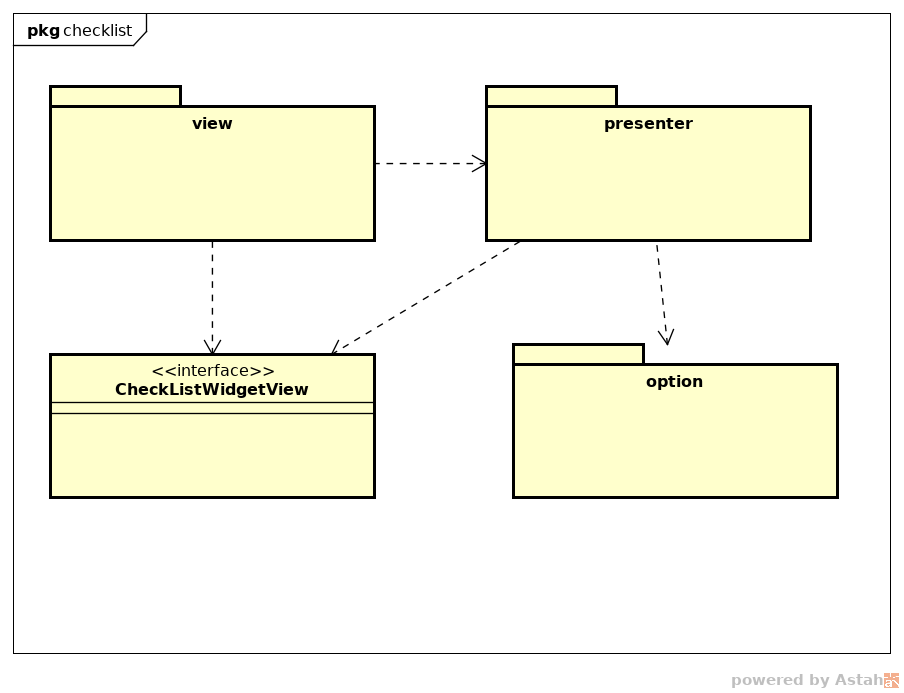
\includegraphics[scale=0.5]{Sezioni/Packages/SDK/component_widget_checklist.png}
	\caption{Monolith::component::widget::checklist}
\end{figure}
\begin{itemize}
	\item{\textbf{Descrizione}}: package contenente tutti i packages e le classi che permettono la creazione di un widget checklist.
	\item{\textbf{Package e classi contenuti}}:
	\begin{itemize}
	\item{monolith::component::widget::checklist::view}: package contenente tutte le classi per la view di un widget checklist.
	\item{monolith::component::widget::checklist::presenter}: package contenente tutte le classi per il presenter di un widget checklist.
	\item{monolith::component::widget::checklist::option}: package contenente tutte le classi per le option di un widget checklist.
	\item{monolith::component::widget::CheckListWidgetView}: interfaccia per un widget checklist.
	\end{itemize}

\end{itemize}


\subsubsection{Suddivisione in package  di Monolith::component::widget::checklist::view}
\label{monolith::component::widget::checklist::view}
\begin{figure}[H]
	\centering
	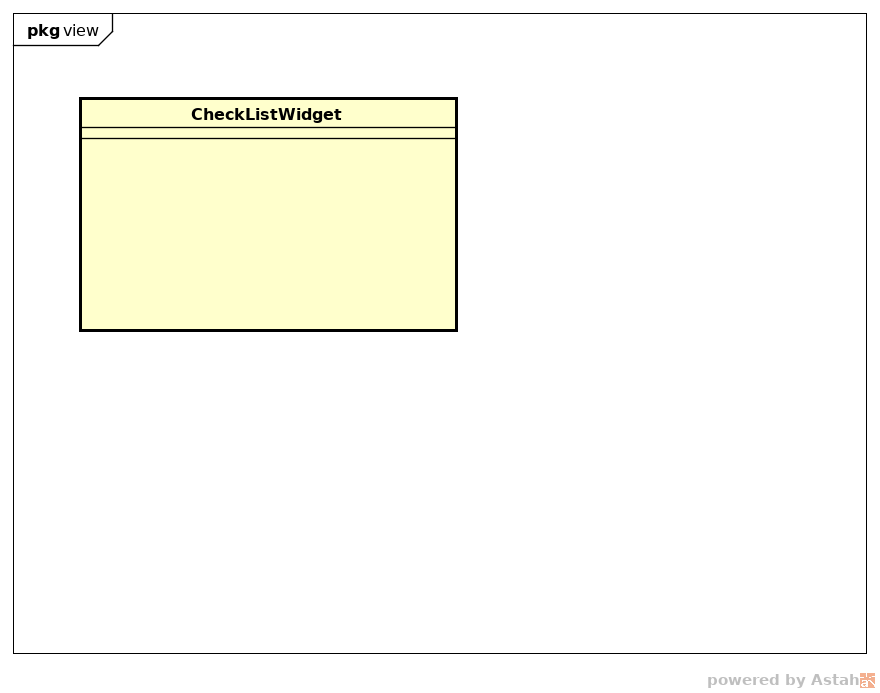
\includegraphics[scale=0.5]{Sezioni/Packages/SDK/component_widget_checklist_view.png}
	\caption{monolith::component::widget::checklist::view}
\end{figure}
\begin{itemize}
	\item{\textbf{Descrizione}}: package contenente la classe view per creare un widget checklist.
	\item{\textbf{Classi contenuti}}:
	\begin{itemize}
	\item{monolith::component::widget::checklist::view::CheckListWidget}: classe view per la creazione di un widget checklist.
	\end{itemize}
\end{itemize}


\subsubsection{Suddivisione in package  di Monolith::component::widget::checklist::presenter}
\label{monolith::component::widget::checklist::presenter}
\begin{figure}[H]
	\centering
	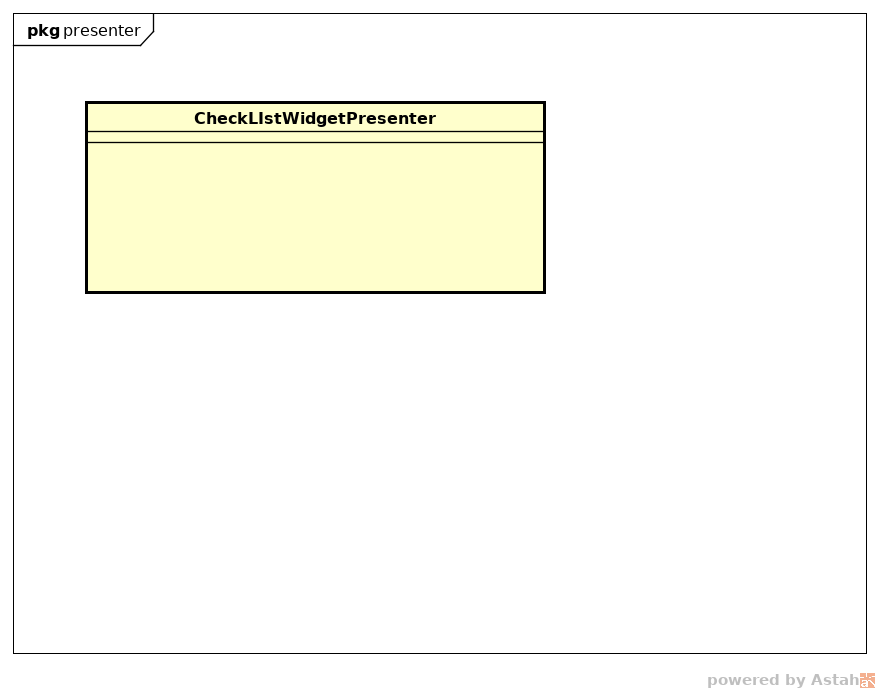
\includegraphics[scale=0.5]{Sezioni/Packages/SDK/component_widget_checklist_presenter.png}
	\caption{onolith::component::widget::checklist::presenter}
\end{figure}
\begin{itemize}
	\item{\textbf{Descrizione}}: package contenente la classe presenter per creare un widget checklist.
	\item{\textbf{Classi contenuti}}:
	\begin{itemize}
	\item{monolith::component::widget::checklist::presenter::CheckLIstWidgetPresenter}: classe presenter per la creazione di un widget checklist.
	\end{itemize}
\end{itemize}



\subsubsection{Suddivisione in package  di Monolith::component::widget::checklist::option}
\label{monolith::component::widget::checklist::option}
\begin{figure}[H]
	\centering
	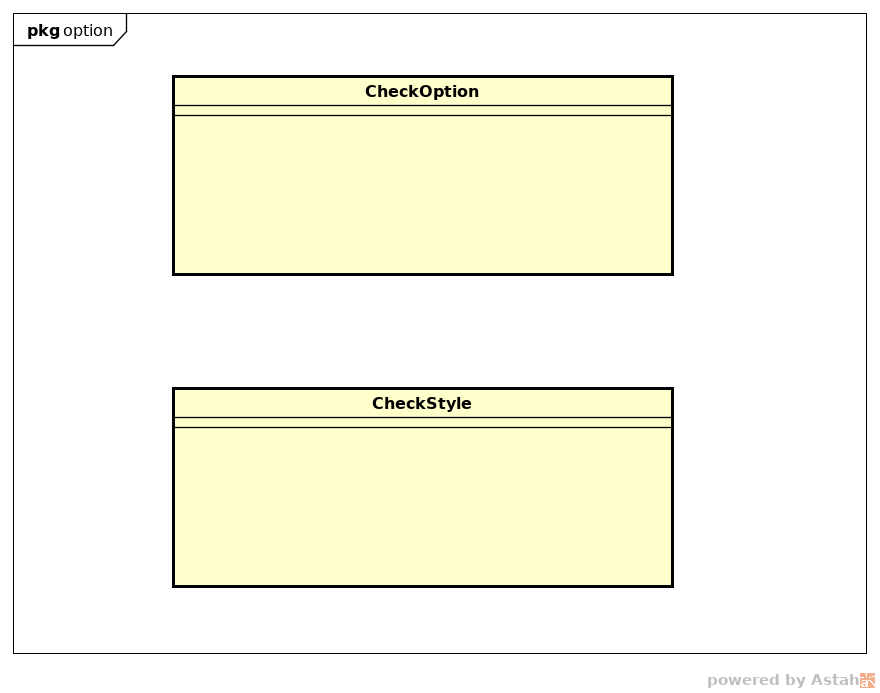
\includegraphics[scale=0.5]{Sezioni/Packages/SDK/component_widget_checklist_option.png}
	\caption{onolith::component::widget::checklist::option}
\end{figure}
\begin{itemize}
	\item{\textbf{Descrizione}}: package contenente le classi option per creare un widget checklist.
	\item{\textbf{Classi contenuti}}:
	\begin{itemize}
	\item{monolith::component::widget::checklist::option::CheckOption}: classe per la modifica della proprietà di spunta del widget checklist.
	\item{monolith::component::widget::checklist::option::CheckStyle}: classe per la modifica della grafica di spunta del widget checklist.
	\end{itemize}
\end{itemize}


\subsubsection{Suddivisione in package  di Monolith::component::widget::image}
\label{Monolith::component::widget::image}
\begin{figure}[H]
	\centering
	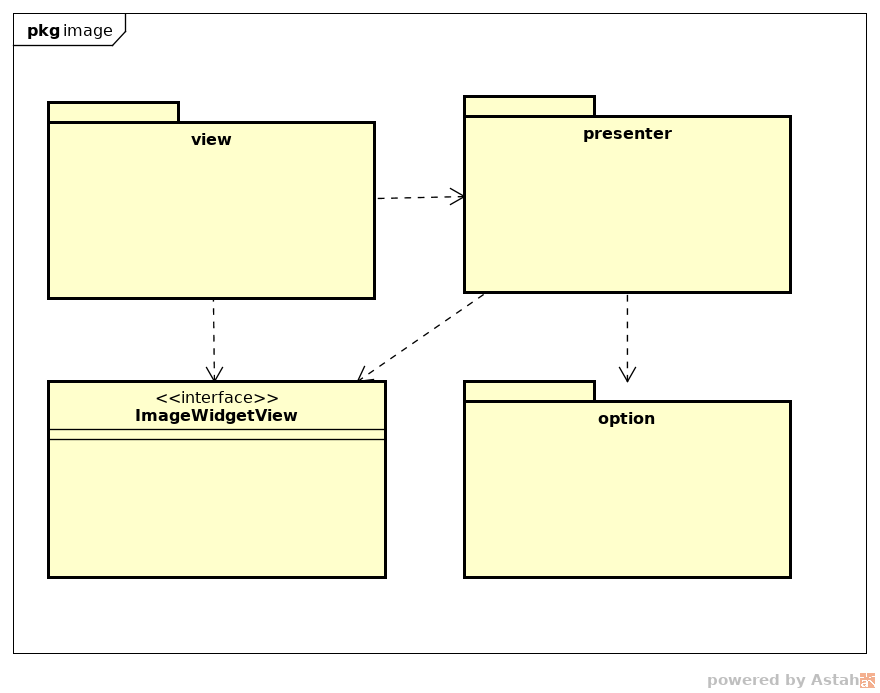
\includegraphics[scale=0.5]{Sezioni/Packages/SDK/component_widget_image.png}
	\caption{Monolith::component::widget::image}
\end{figure}
\begin{itemize}
	\item{\textbf{Descrizione}}: package contenente tutti i packages e le classi che permettono la creazione di un widget image.
	\item{\textbf{Package e classi contenuti}}:
	\begin{itemize}
	\item{monolith::component::widget::image::view}: package contenente tutte le classi per la view di un widget image.
	\item{monolith::component::widget::image::presenter}: package contenente tutte le classi per il presenter di un widget image.
	\item{monolith::component::widget::image::option}: package contenente tutte le classi per le option di un widget image.
	\item{monolith::component::widget::image:ImageWidgetView}: interfaccia per un widget image.
	\end{itemize}

\end{itemize}


\subsubsection{Suddivisione in package  di Monolith::component::widget::image::view}
\label{monolith::component::widget::image::view}
\begin{figure}[H]
	\centering
	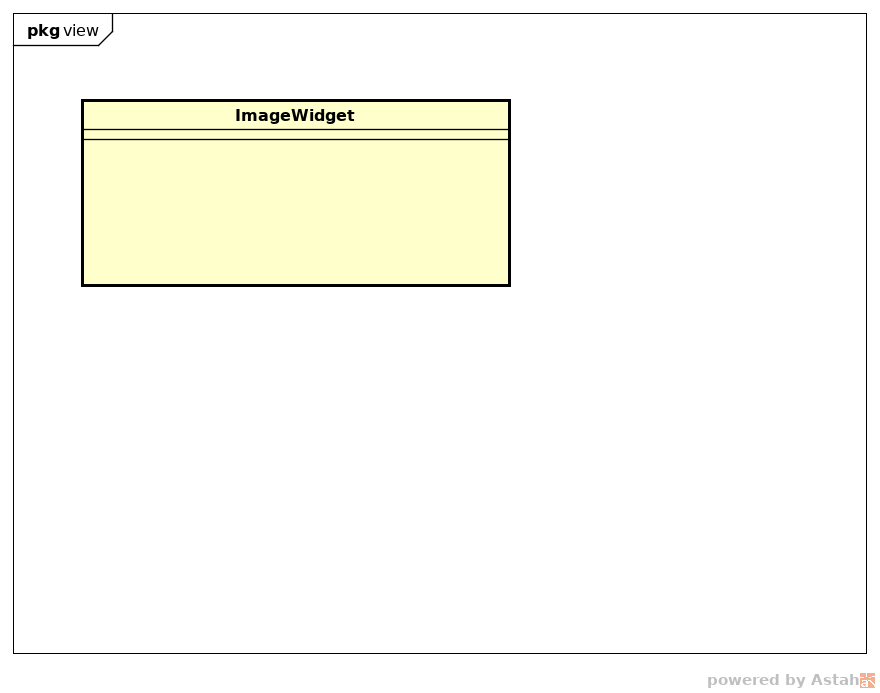
\includegraphics[scale=0.5]{Sezioni/Packages/SDK/component_widget_image_view.png}
	\caption{monolith::component::widget::image::view}
\end{figure}
\begin{itemize}
	\item{\textbf{Descrizione}}: package contenente la classe view per creare un widget image.
	\item{\textbf{Classi contenuti}}:
	\begin{itemize}
	\item{monolith::component::widget::checklist::view::ImageWidget}: classe view per la creazione di un widget image.
	\end{itemize}
\end{itemize}


\subsubsection{Suddivisione in package  di Monolith::component::widget::image::presenter}
\label{monolith::component::widget::image::presenter}
\begin{figure}[H]
	\centering
	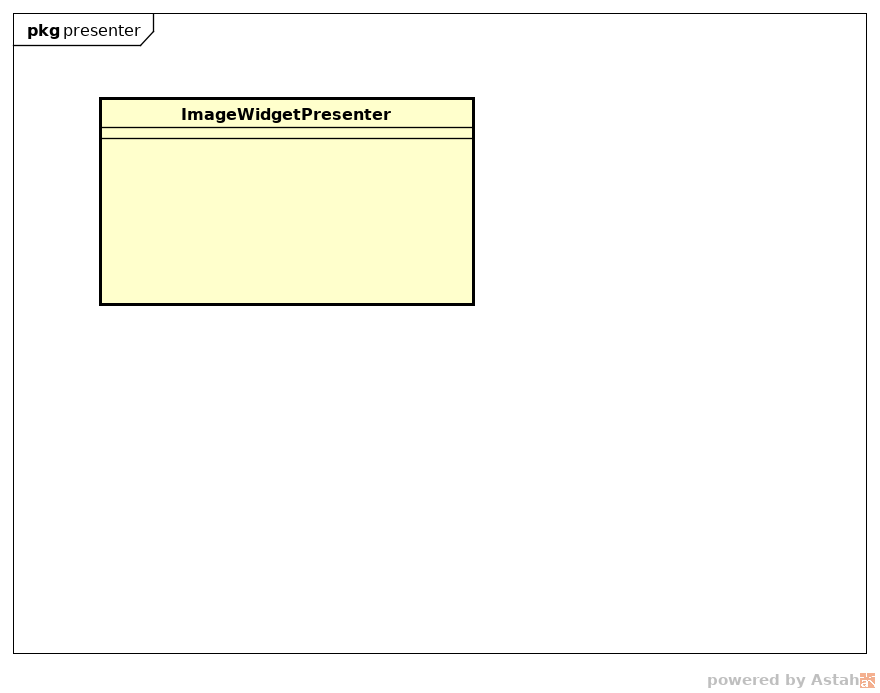
\includegraphics[scale=0.5]{Sezioni/Packages/SDK/component_widget_image_presenter.png}
	\caption{monolith::component::widget::image::presenter}
\end{figure}
\begin{itemize}
	\item{\textbf{Descrizione}}: package contenente la classe presenter per creare un widget image.
	\item{\textbf{Classi contenuti}}:
	\begin{itemize}
	\item{monolith::component::widget::checklist::image::ImageWidgetPresenter}: classe presenter per la creazione di un widget image.
	\end{itemize}
\end{itemize}



\subsubsection{Suddivisione in package  di Monolith::component::widget::image::option}
\label{onolith::component::widget::image::option}
\begin{figure}[H]
	\centering
	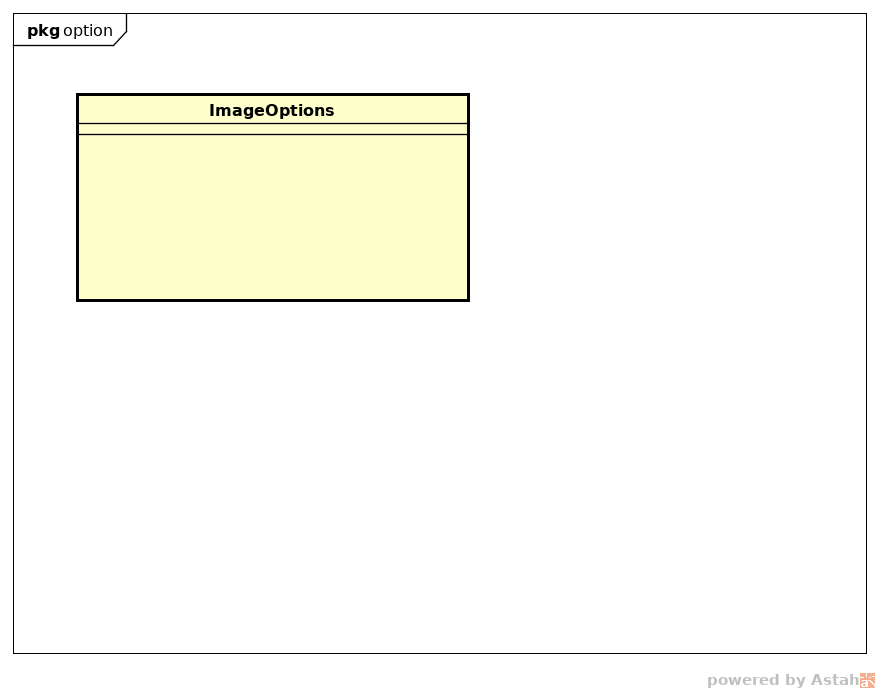
\includegraphics[scale=0.5]{Sezioni/Packages/SDK/component_widget_image_option.png}
	\caption{onolith::component::widget::image::option}
\end{figure}
\begin{itemize}
	\item{\textbf{Descrizione}}: package contenente le classi option per creare un widget image.
	\item{\textbf{Classi contenuti}}:
	\begin{itemize}
	\item{monolith::component::widget::image::option::ImageOptions}: classe per la modifica della proprietà dell'immagine del widget image.
	\end{itemize}
\end{itemize}


\subsubsection{Suddivisione in package  di Monolith::component::widget::list}
\label{Monolith::component::widget::list}
\begin{figure}[H]
	\centering
	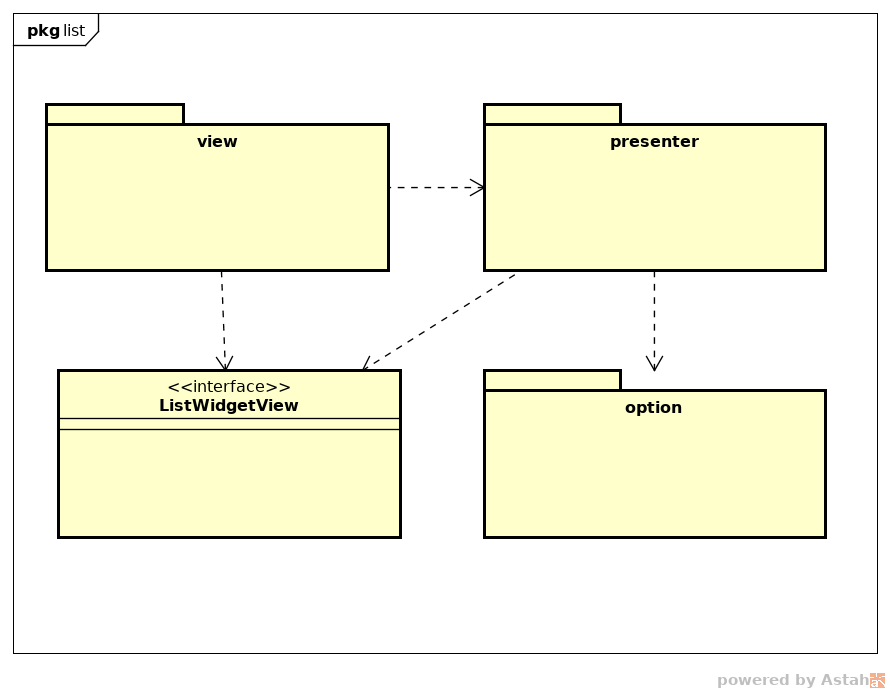
\includegraphics[scale=0.5]{Sezioni/Packages/SDK/component_widget_list.png}
	\caption{Monolith::component::widget::list}
\end{figure}
\begin{itemize}
	\item{\textbf{Descrizione}}: package contenente tutti i packages e le classi che permettono la creazione di un widget list.
	\item{\textbf{Package e classi contenuti}}:
	\begin{itemize}
	\item{monolith::component::widget::list::view}: package contenente tutte le classi per la view di un widget list.
	\item{monolith::component::widget::list::presenter}: package contenente tutte le classi per il presenter di un widget list.
	\item{monolith::component::widget::list::option}: package contenente tutte le classi per le option di un widget list.
	\item{monolith::component::widget::list:ListWidgetView}: interfaccia per un widget .
	\end{itemize}

\end{itemize}


\subsubsection{Suddivisione in package  di Monolith::component::widget::list::view}
\label{monolith::component::widget::list::view}
\begin{figure}[H]
	\centering
	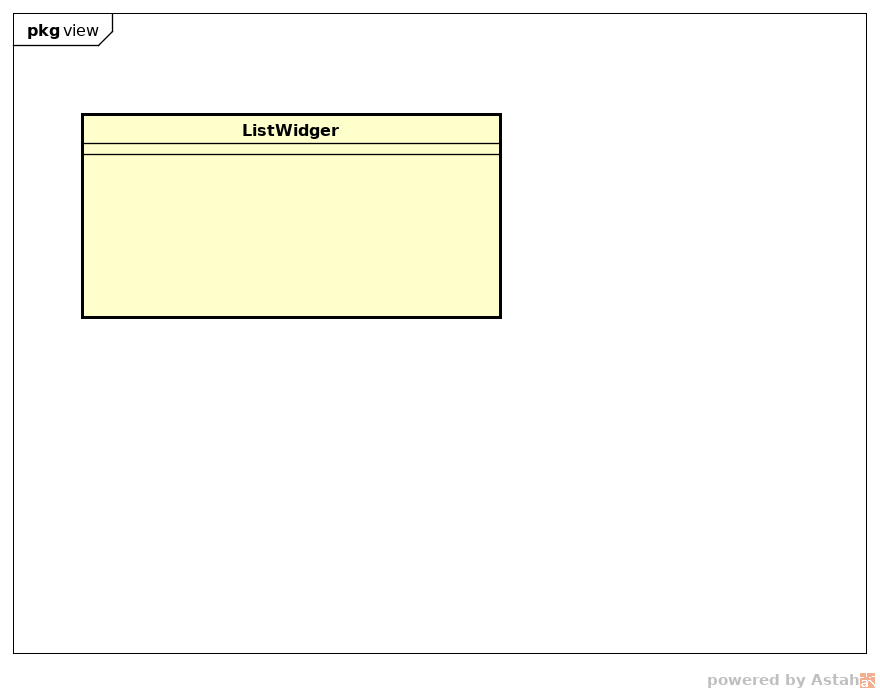
\includegraphics[scale=0.5]{Sezioni/Packages/SDK/component_widget_list_view.png}
	\caption{monolith::component::widget::list::view}
\end{figure}
\begin{itemize}
	\item{\textbf{Descrizione}}: package contenente la classe view per creare un widget list.
	\item{\textbf{Classi contenuti}}:
	\begin{itemize}
	\item{monolith::component::widget::list::view::ListWidger}: classe view per la creazione di un widget image.
	\end{itemize}
\end{itemize}


\subsubsection{Suddivisione in package  di Monolith::component::widget::list::presenter}
\label{monolith::component::widget::list::presenter}
\begin{figure}[H]
	\centering
	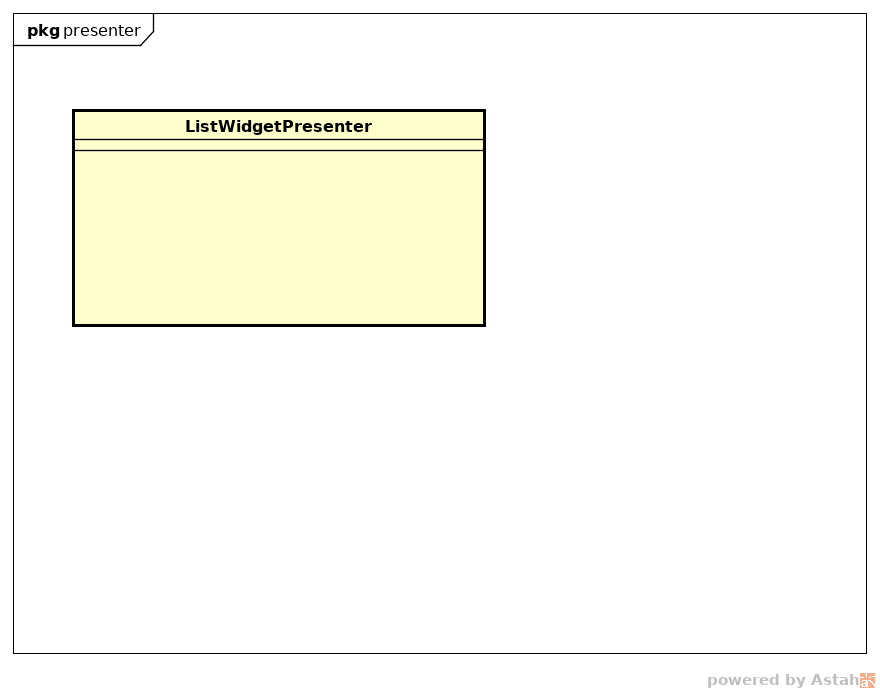
\includegraphics[scale=0.5]{Sezioni/Packages/SDK/component_widget_list_presenter.png}
	\caption{monolith::component::widget::list::presenter}
\end{figure}
\begin{itemize}
	\item{\textbf{Descrizione}}: package contenente la classe presenter per creare un widget list.
	\item{\textbf{Classi contenuti}}:
	\begin{itemize}
	\item{monolith::component::widget::list::image::ListWidgetPresenter}: classe presenter per la creazione di un widget list.
	\end{itemize}
\end{itemize}



\subsubsection{Suddivisione in package  di Monolith::component::widget::list::option}
\label{monolith::component::widget::list::option}
\begin{figure}[H]
	\centering
	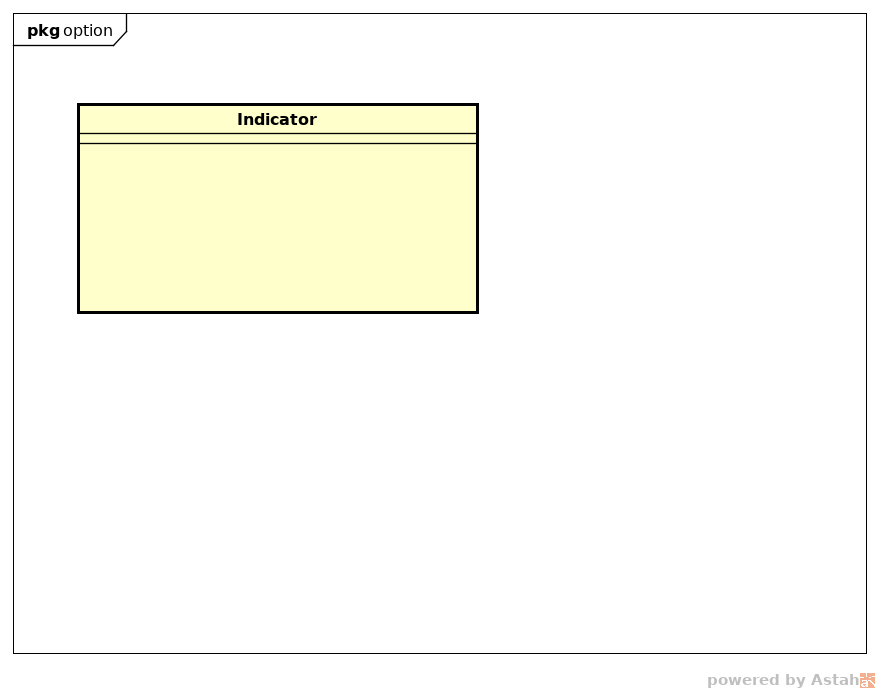
\includegraphics[scale=0.5]{Sezioni/Packages/SDK/component_widget_list_option.png}
	\caption{onolith::component::widget::list::option}
\end{figure}
\begin{itemize}
	\item{\textbf{Descrizione}}: package contenente le classi option per creare un widget list.
	\item{\textbf{Classi contenuti}}:
	\begin{itemize}
	\item{monolith::component::widget::list::option::Indicator}: classe per la modifica della proprietà dell'indicatore del singolo item del widget list.
	\end{itemize}
\end{itemize}




\subsubsection{Suddivisione in package  di Monolith::component::widget::text}
\label{Monolith::component::widget::text}
\begin{figure}[H]
	\centering
	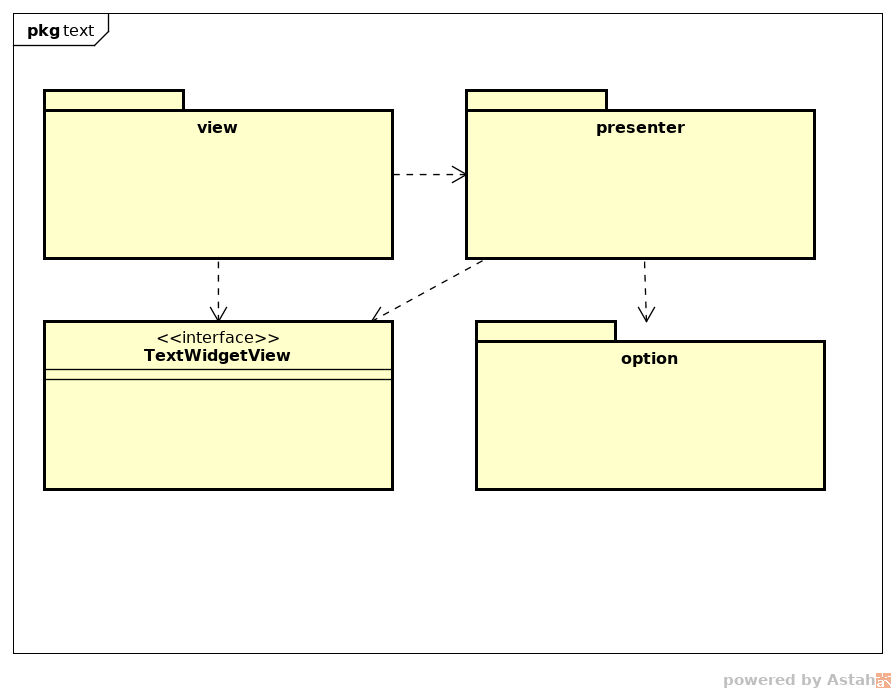
\includegraphics[scale=0.5]{Sezioni/Packages/SDK/component_widget_text.png}
	\caption{Monolith::component::widget::text}
\end{figure}
\begin{itemize}
	\item{\textbf{Descrizione}}: package contenente tutti i packages e le classi che permettono la creazione di un widget text.
	\item{\textbf{Package e classi contenuti}}:
	\begin{itemize}
	\item{monolith::component::widget::text::view}: package contenente tutte le classi per la view di un widget text.
	\item{monolith::component::widget::text::presenter}: package contenente tutte le classi per il presenter di un widget text.
	\item{monolith::component::widget::text::option}: package contenente tutte le classi per le option di un widget text.
	\item{monolith::component::widget::text:TextWidgetView}: interfaccia per un widget text.
	\end{itemize}

\end{itemize}


\subsubsection{Suddivisione in package  di Monolith::component::widget::text::view}
\label{monolith::component::widget::text::view}
\begin{figure}[H]
	\centering
	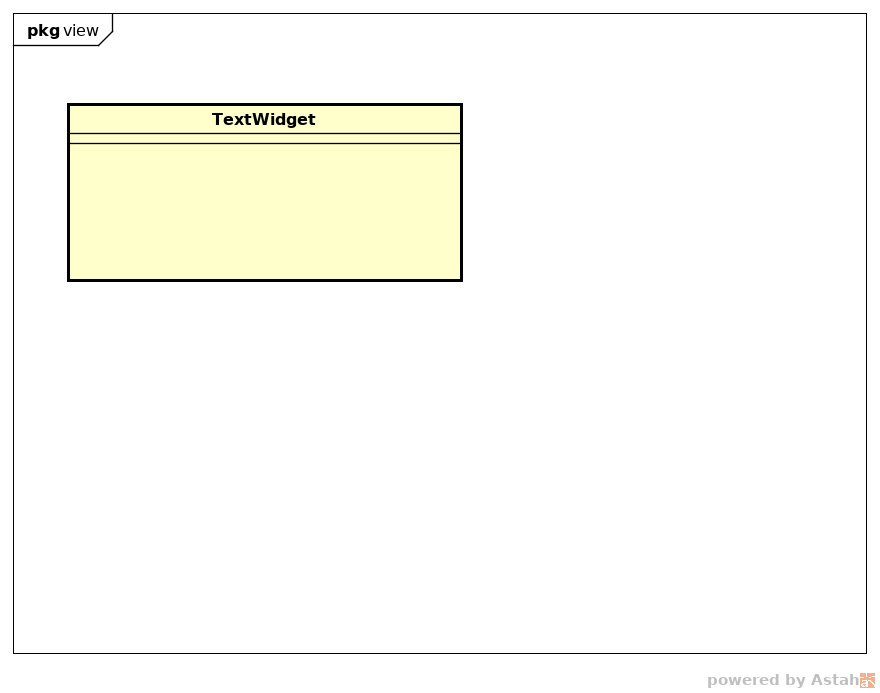
\includegraphics[scale=0.5]{Sezioni/Packages/SDK/component_widget_text_view.png}
	\caption{monolith::component::widget::text::view}
\end{figure}
\begin{itemize}
	\item{\textbf{Descrizione}}: package contenente la classe view per creare un widget text.
	\item{\textbf{Classi contenuti}}:
	\begin{itemize}
	\item{monolith::component::widget::text::view::TextWidget}: classe view per la creazione di un widget text.
	\end{itemize}
\end{itemize}


\subsubsection{Suddivisione in package  di Monolith::component::widget::text::presenter}
\label{monolith::component::widget::text::presenter}
\begin{figure}[H]
	\centering
	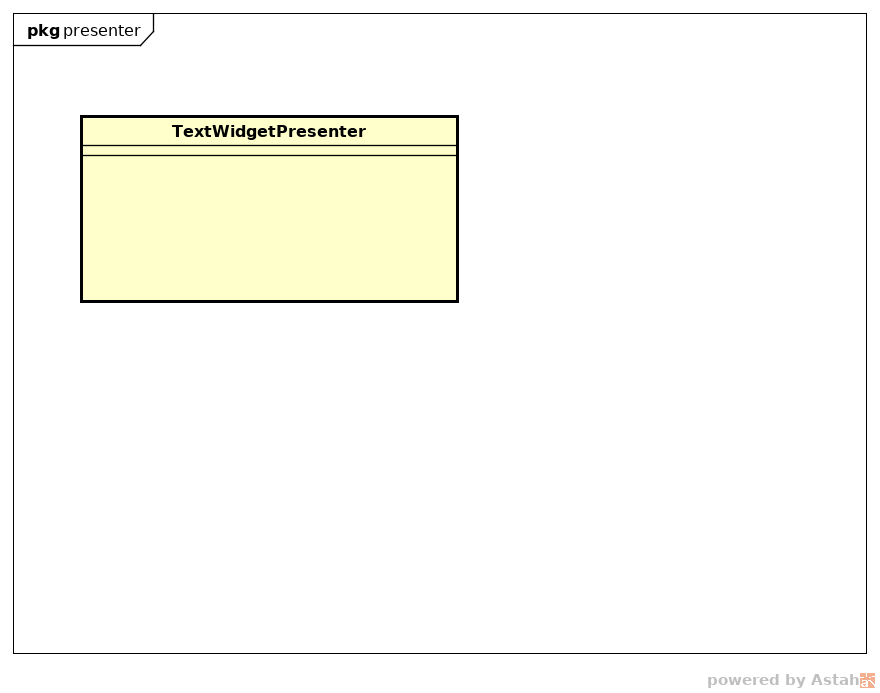
\includegraphics[scale=0.5]{Sezioni/Packages/SDK/component_widget_text_presenter.png}
	\caption{monolith::component::widget::text::presenter}
\end{figure}
\begin{itemize}
	\item{\textbf{Descrizione}}: package contenente la classe presenter per creare un widget text.
	\item{\textbf{Classi contenuti}}:
	\begin{itemize}
	\item{monolith::component::widget::text::TextWidgetPresenter}: classe presenter per la creazione di un widget text.
	\end{itemize}
\end{itemize}



\subsubsection{Suddivisione in package  di Monolith::component::widget::text::option}
\label{monolith::component::widget::text::option}
\begin{figure}[H]
	\centering
	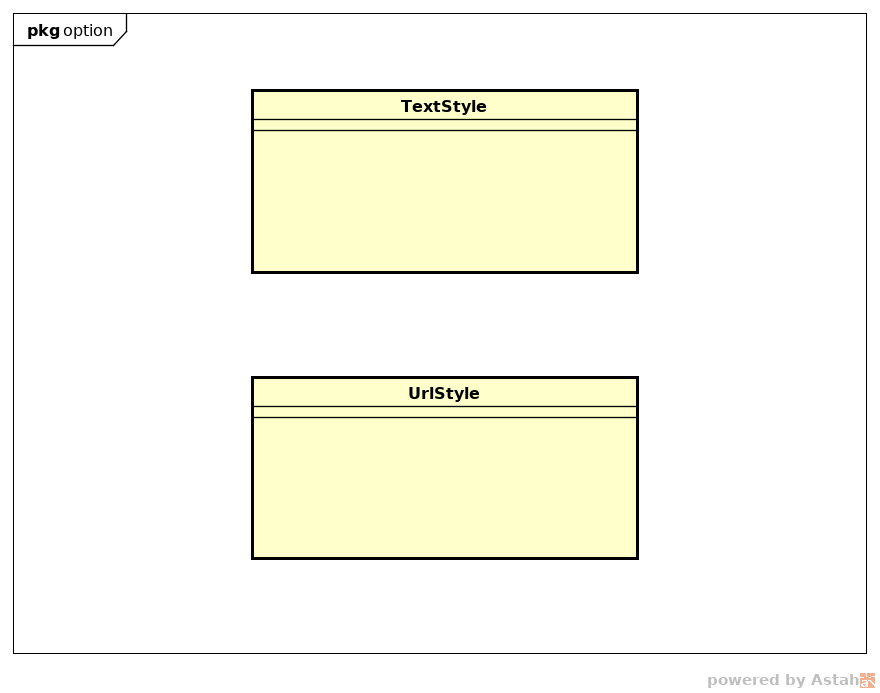
\includegraphics[scale=0.5]{Sezioni/Packages/SDK/component_widget_text_option.png}
	\caption{onolith::component::widget::text::option}
\end{figure}
\begin{itemize}
	\item{\textbf{Descrizione}}: package contenente le classi option per creare un widget text.
	\item{\textbf{Classi contenuti}}:
	\begin{itemize}
	\item{monolith::component::widget::text::option::TextStyle}: classe per la modifica dello stile di testo del widget text.
	\item{monolith::component::widget::text::option::UrlStyle}: classe per la modifica dello stile dell' url del widget text.
	\end{itemize}
\end{itemize}
\end{comment}